\chapter{Results}
         \section{Data and Prediction Agreement in Preselection Region}
         Here a preselection is shown to demonstrate the agreement between the full data driven predictions and data. This region is composed of the full signal selections with the jet requirements loosened to 2 or more jets from the signal selection of 4. This is done to be able to preserve the b-Tags requirement. What results is a region with almost twice the events of the signal region and slightly enhanced backgrounds, both being useful to help illustrate the agreement of the predictions and data. WZ is a dominant background and thus the reconstructed mass of the Z and the \Mt \ of the W (Figure ~\ref{fig:hmass_3L2b}) are good variables for comparison. Additionally, in the preselection region, it is possible to view a more complete picture of the jet multiplicity (Figure ~\ref{fig:jetmult_3L2b}) which is important as this is used in the full selection. Finally, other distributions such as the lepton \pt \ are shown (Figure ~\ref{fig:hleppt_3L2b}). In the following plots, the irreducible background is taken from pure MC where the events have been scaled by lepton efficiency data to MC scale factors and the similar b-Tagging efficiency scale factors. The luminosity is scaled to that of data. For the data driven predictions, the shape is taken from MC while the normalization of the background is from the data driven predictions in Section ~\ref{sec:datadriven}.

\begin{figure}[h]
\begin{center}
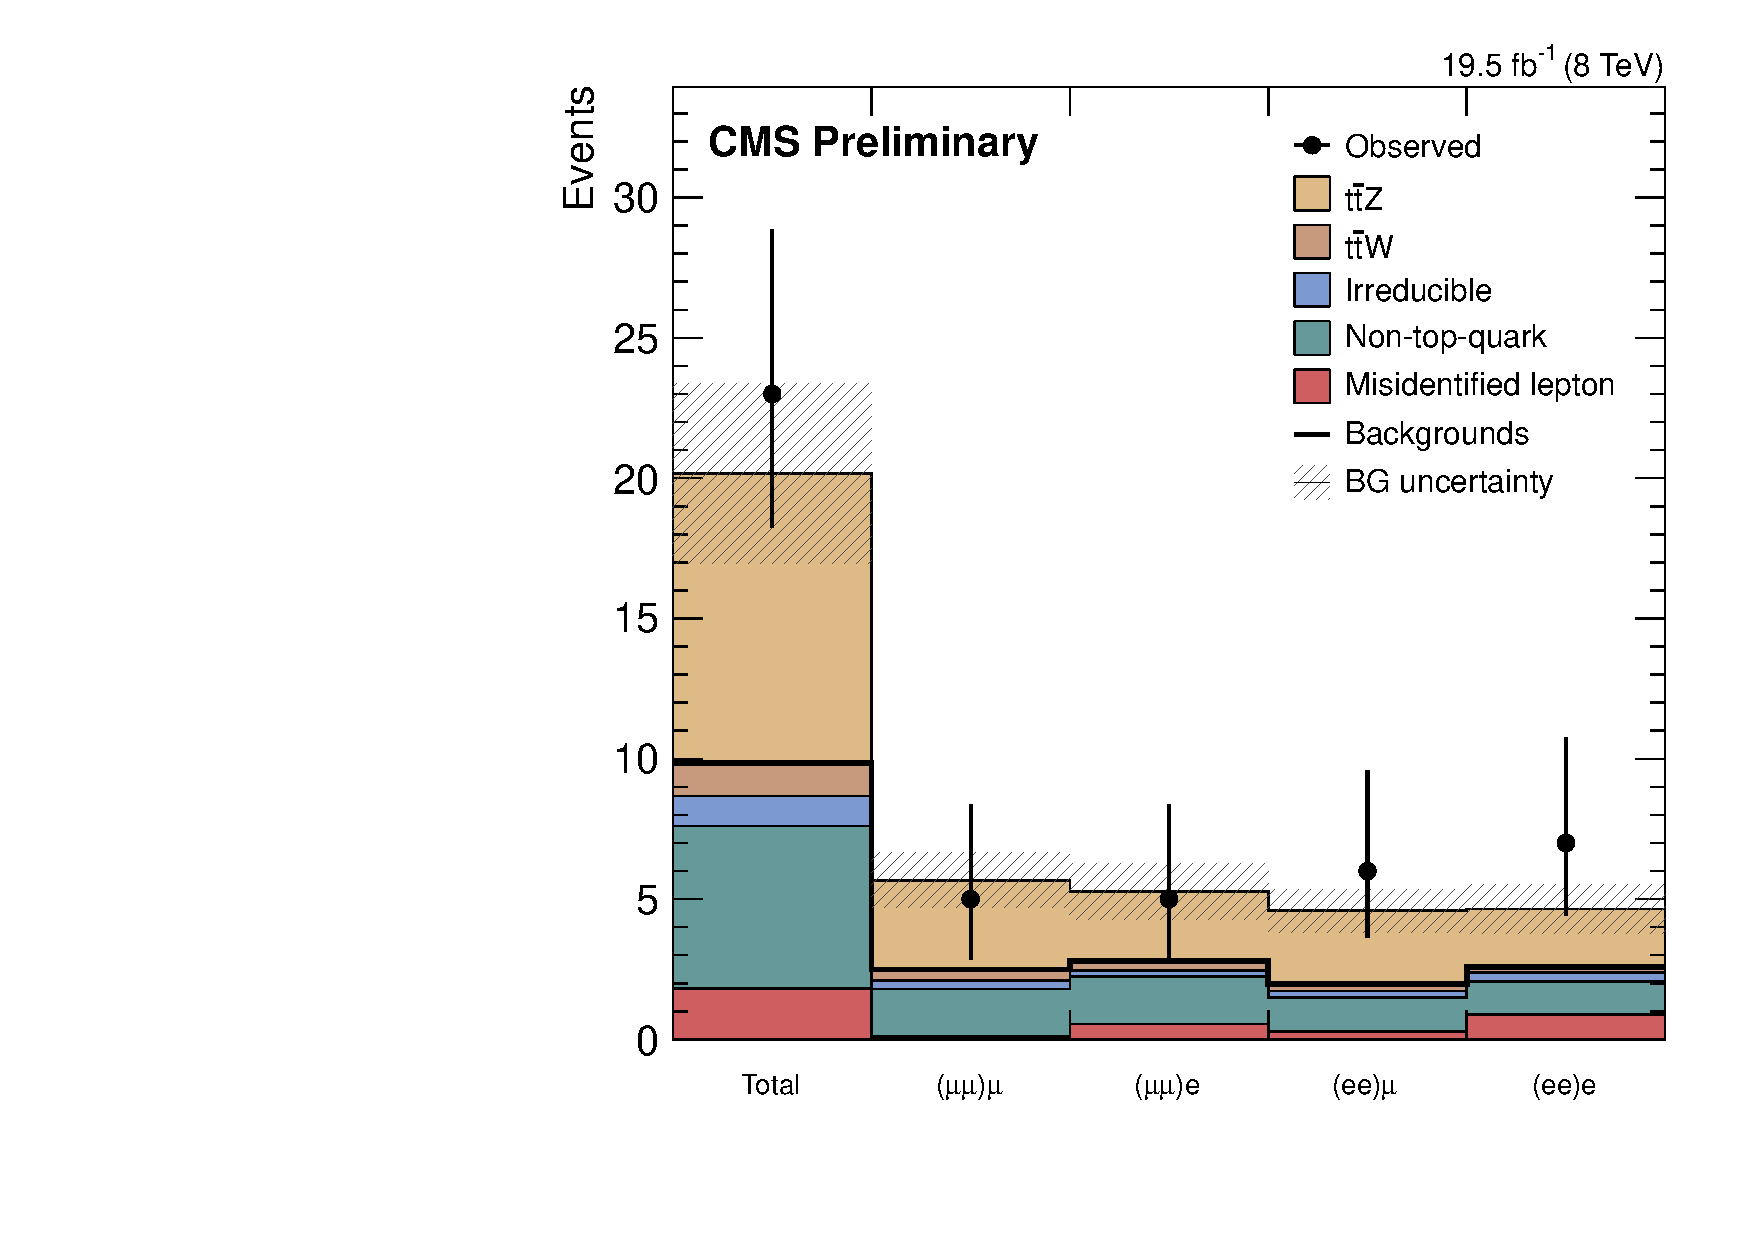
\includegraphics[width=0.48\linewidth]{Figs/Plots_PreSelections/hYields_3L2b.pdf}
\caption{\label{fig:hyields_3L2b}
Yields with channel break down of data and predictions after tri-lepton plus 2 b-Tag selections.
}
\end{center}
\end{figure}

\begin{figure}[h]
\begin{center}
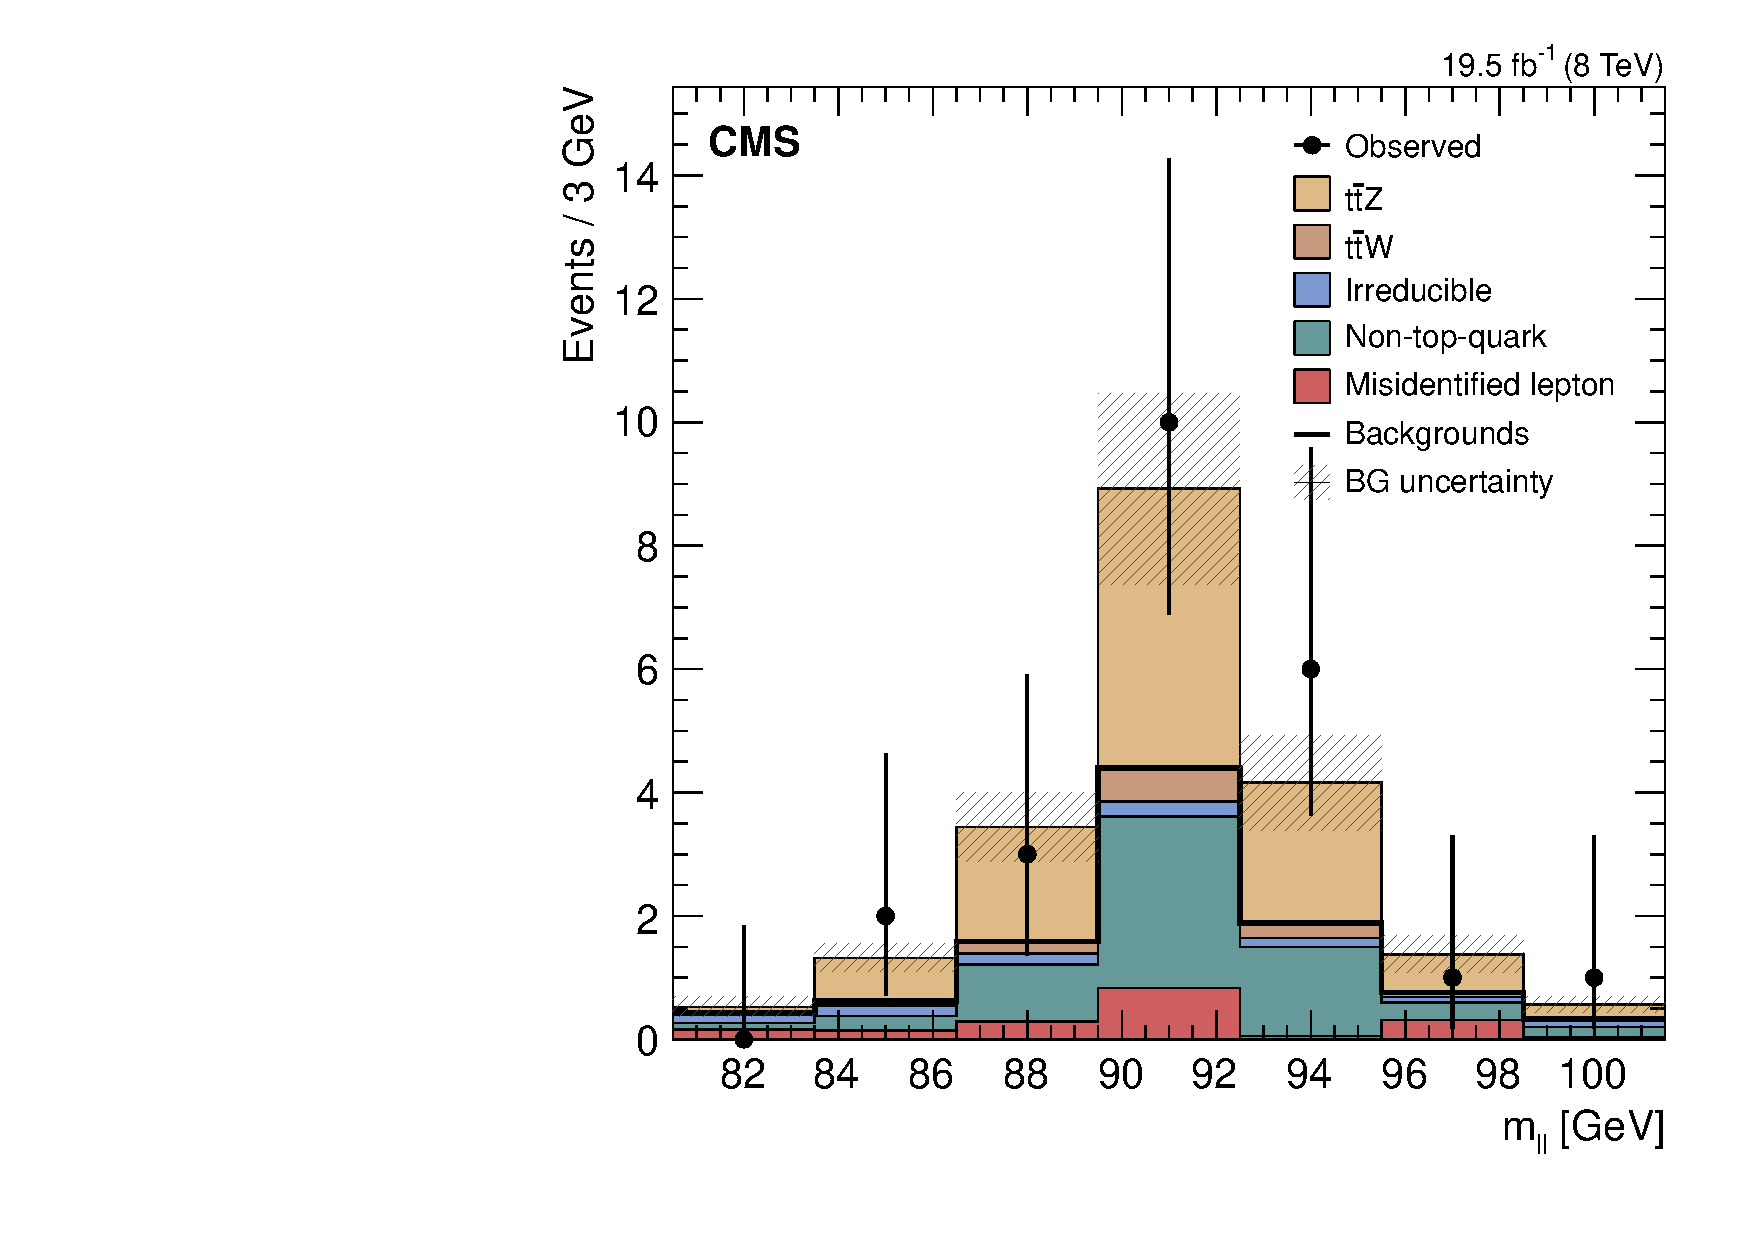
\includegraphics[width=0.48\linewidth]{Figs/Plots_PreSelections/hZMass_3L2b.pdf}
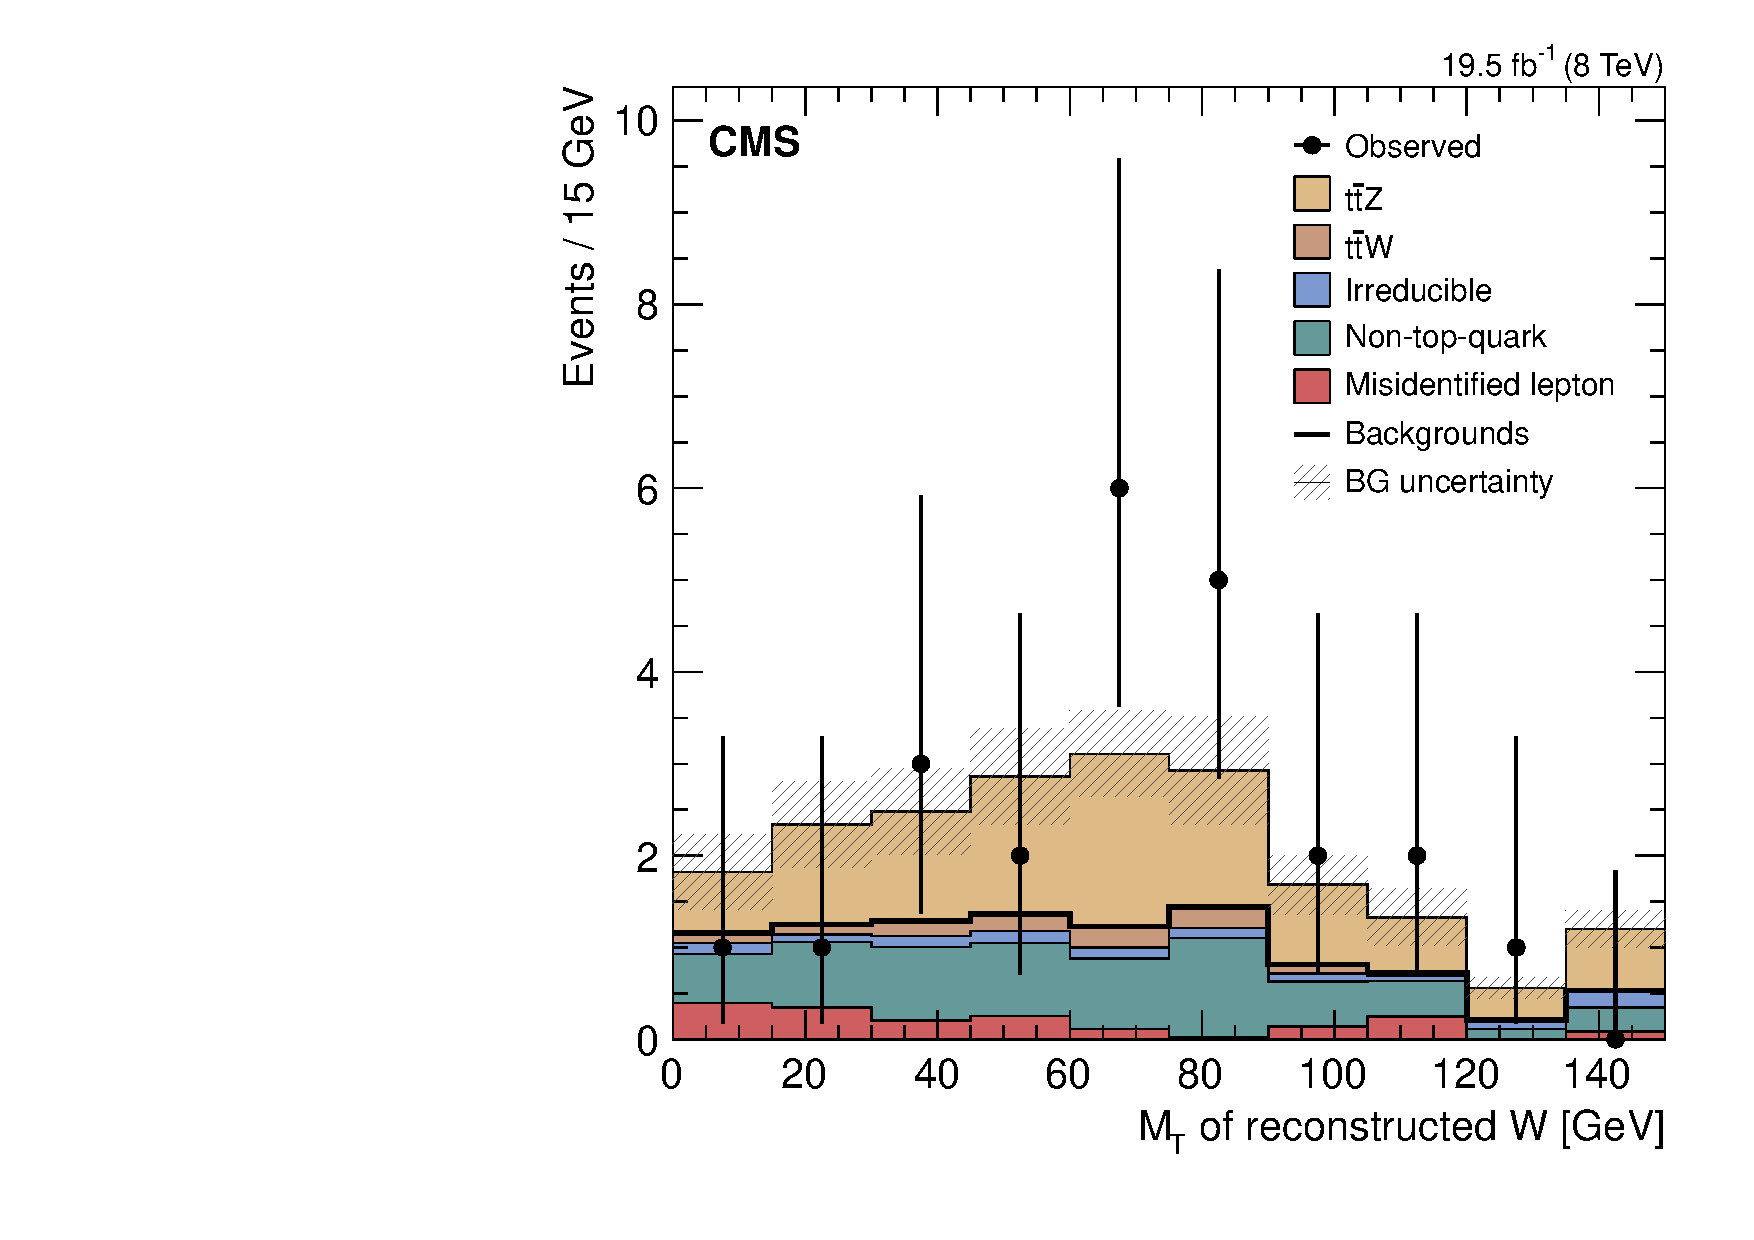
\includegraphics[width=0.48\linewidth]{Figs/Plots_PreSelections/hWMt_3L2b.pdf}
\caption{\label{fig:hmass_3L2b}
Reconstructed mass plots after tri-lepton plus 2 b-Tag selections. Reconstructed Z Mass from lepton pair (Left). Reconstructed W \Mt \ (Right ).
}
\end{center}
\end{figure}

\begin{figure}[h]
\begin{center}
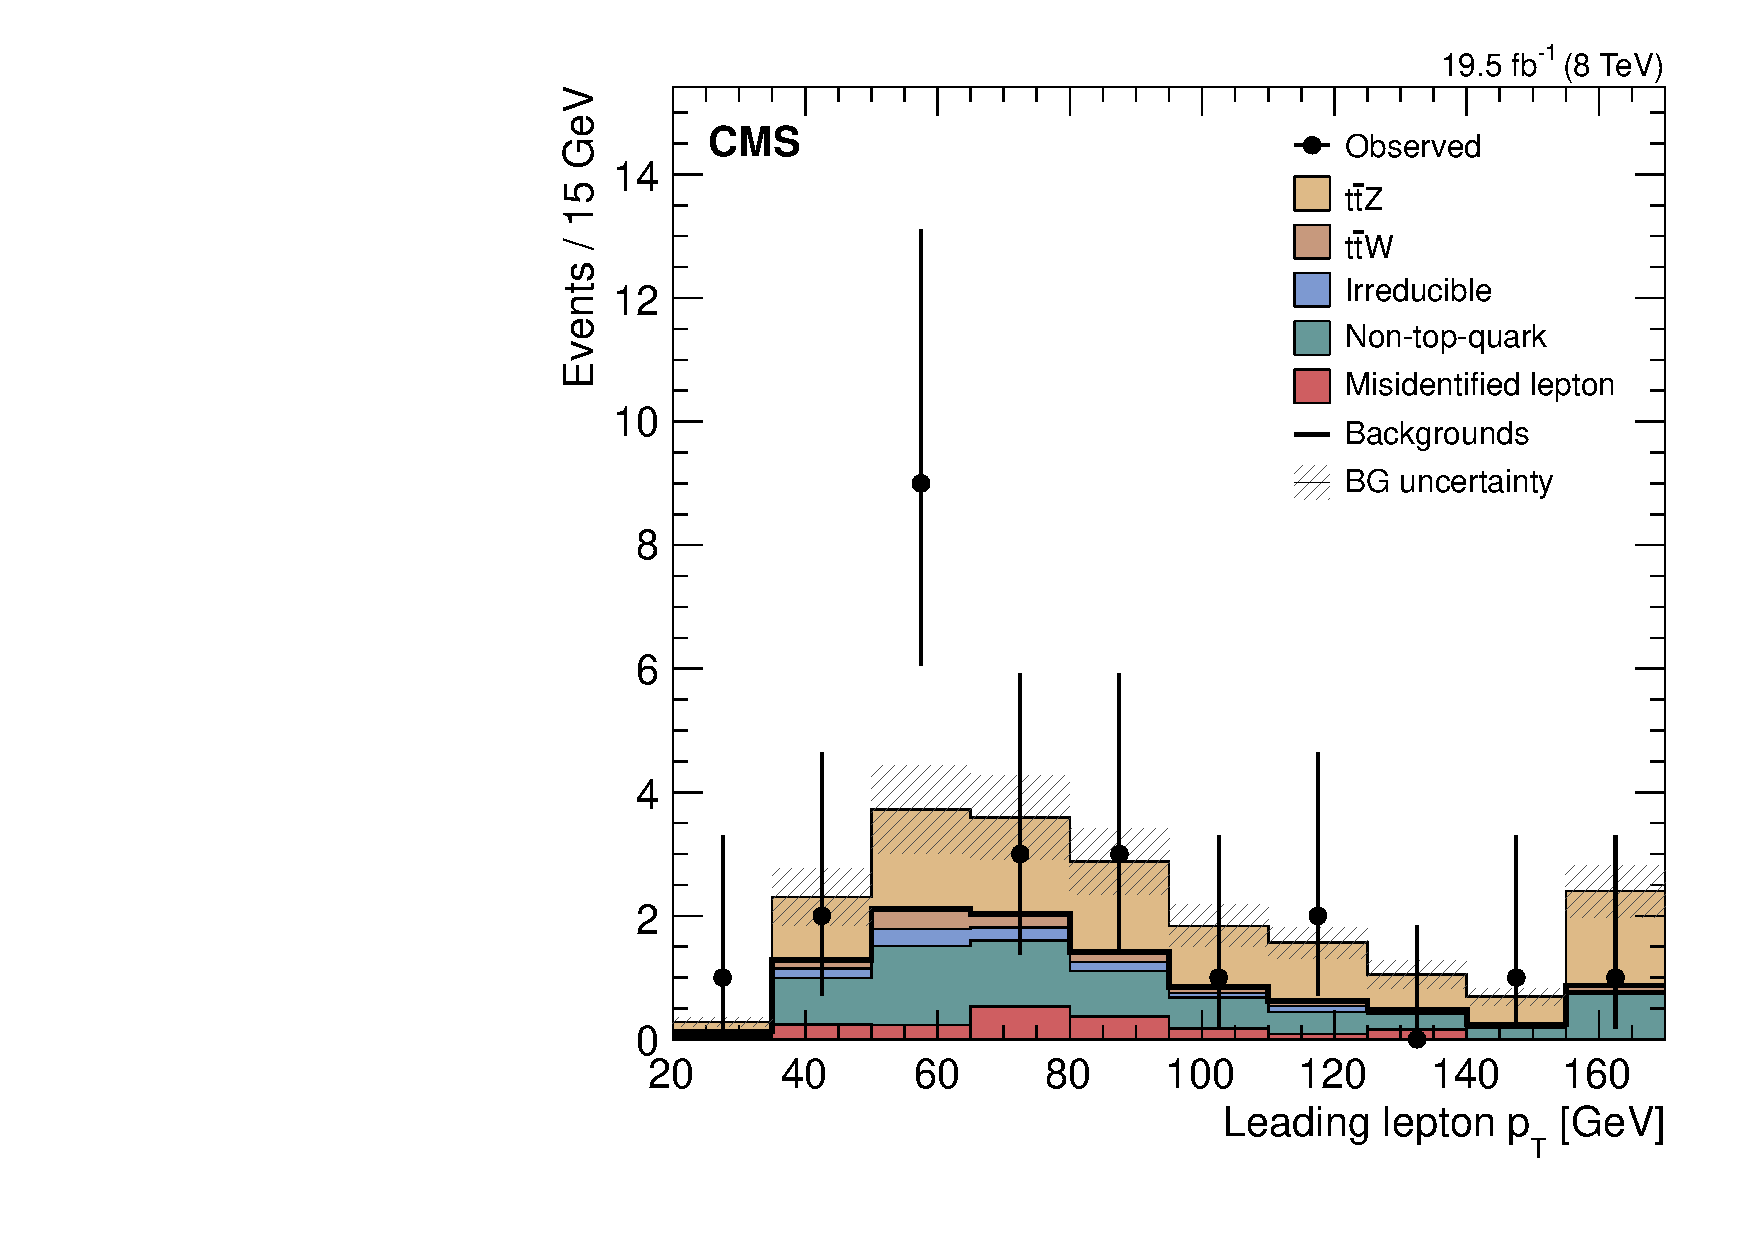
\includegraphics[width=0.48\linewidth]{Figs/Plots_PreSelections/hZLep1Pt_3L2b.pdf}
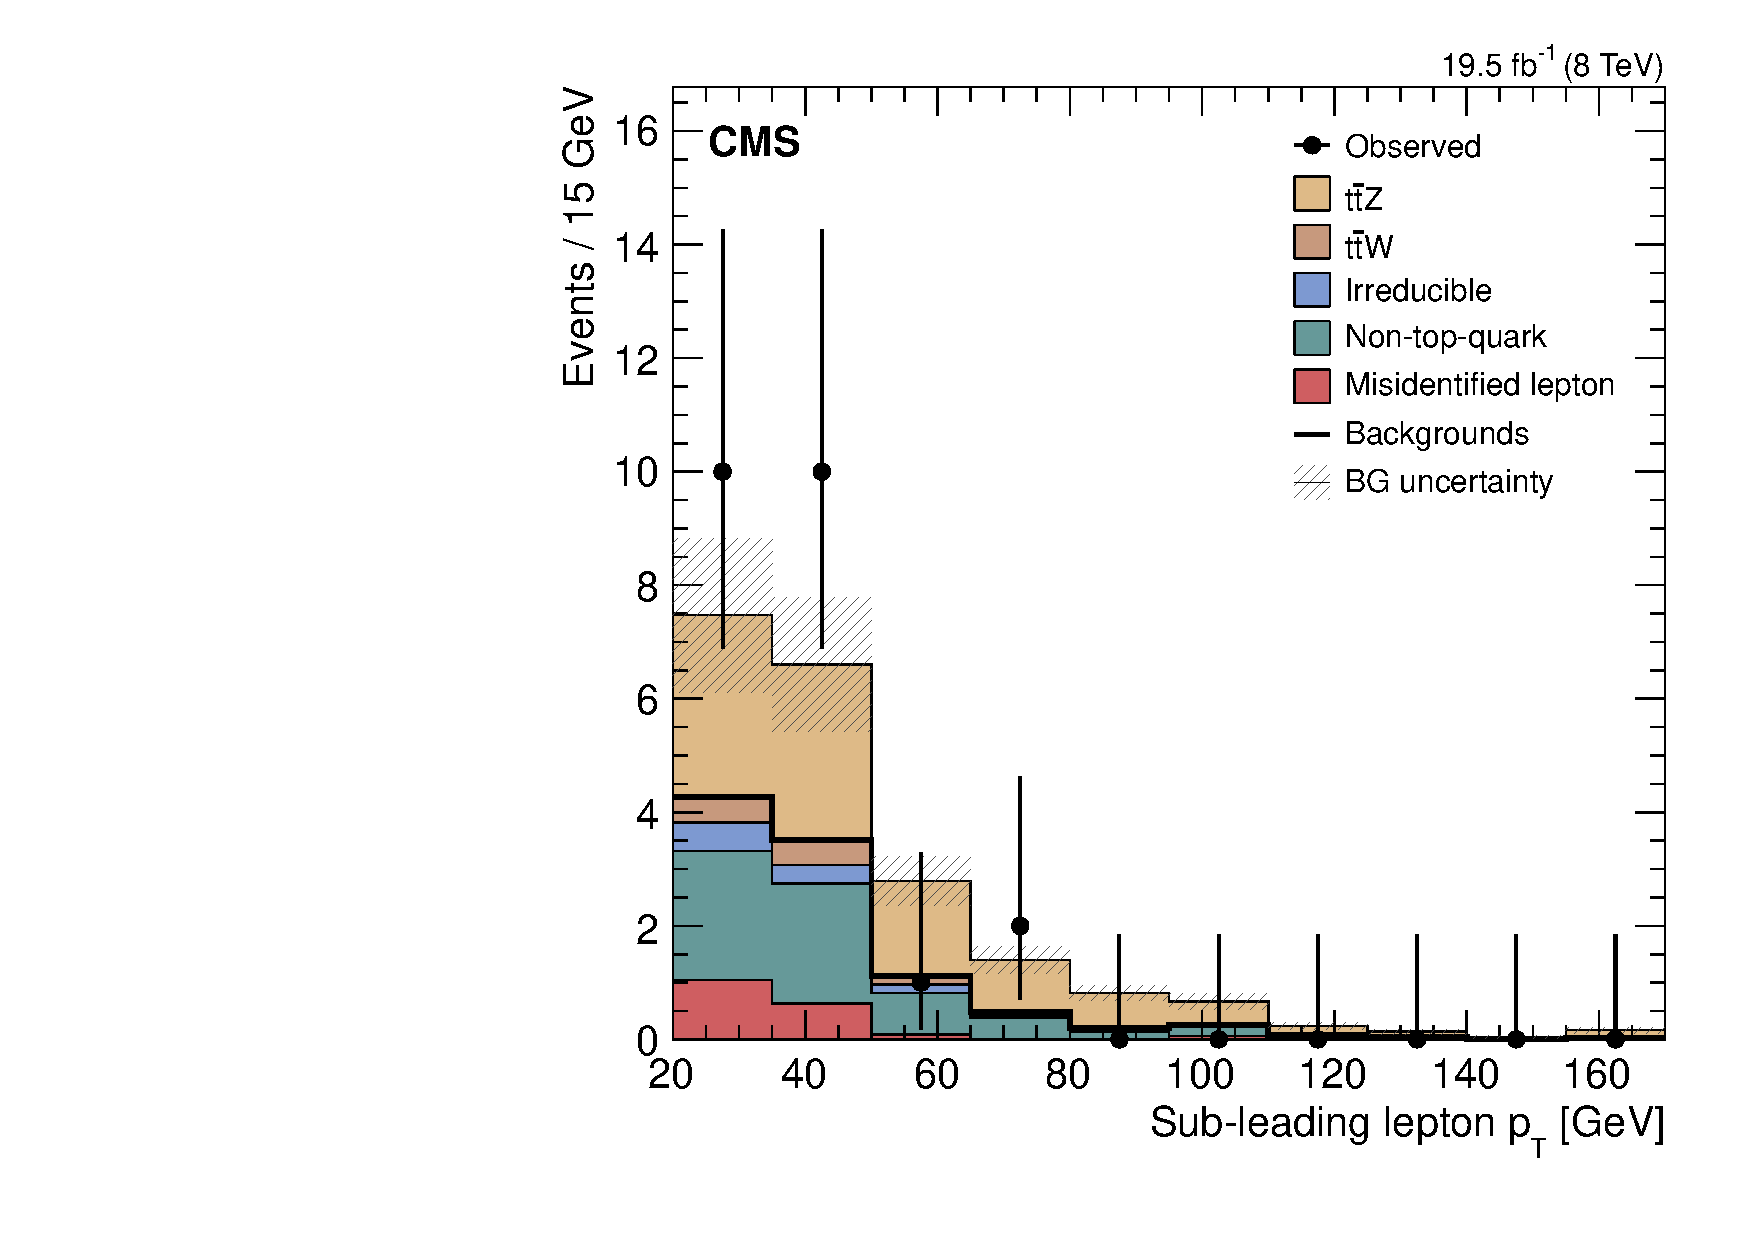
\includegraphics[width=0.48\linewidth]{Figs/Plots_PreSelections/hZLep2Pt_3L2b.pdf}
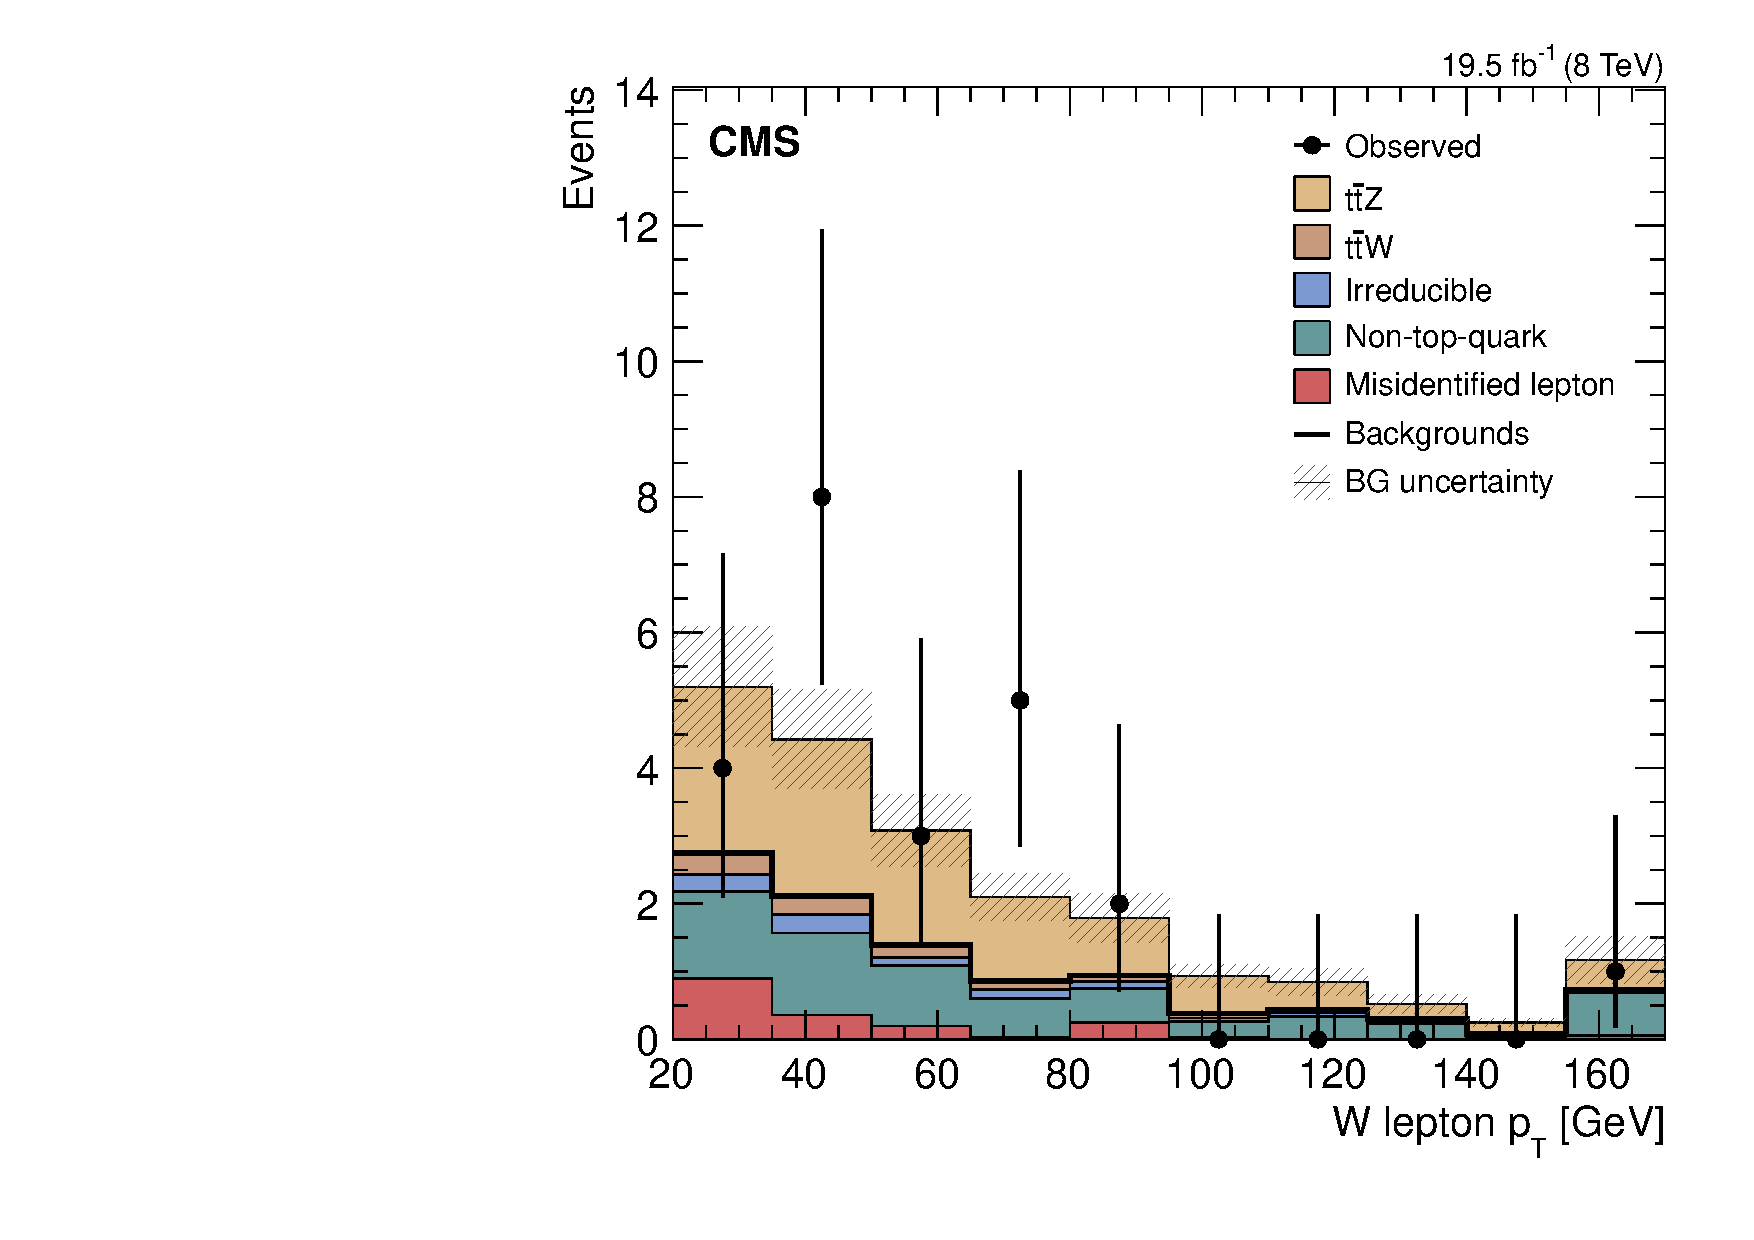
\includegraphics[width=0.48\linewidth]{Figs/Plots_PreSelections/hWLepPt_3L2b.pdf}
\caption{\label{fig:hleppt_3L2b}
PT of the Z and W leptons after tri-lepton plus 2 b-Tag selections. Left: Leading Pt lepton. Right: Trailing Pt lepton. Bottom: W lepton.
}
\end{center}
\end{figure}

\begin{figure}[h]
\begin{center}
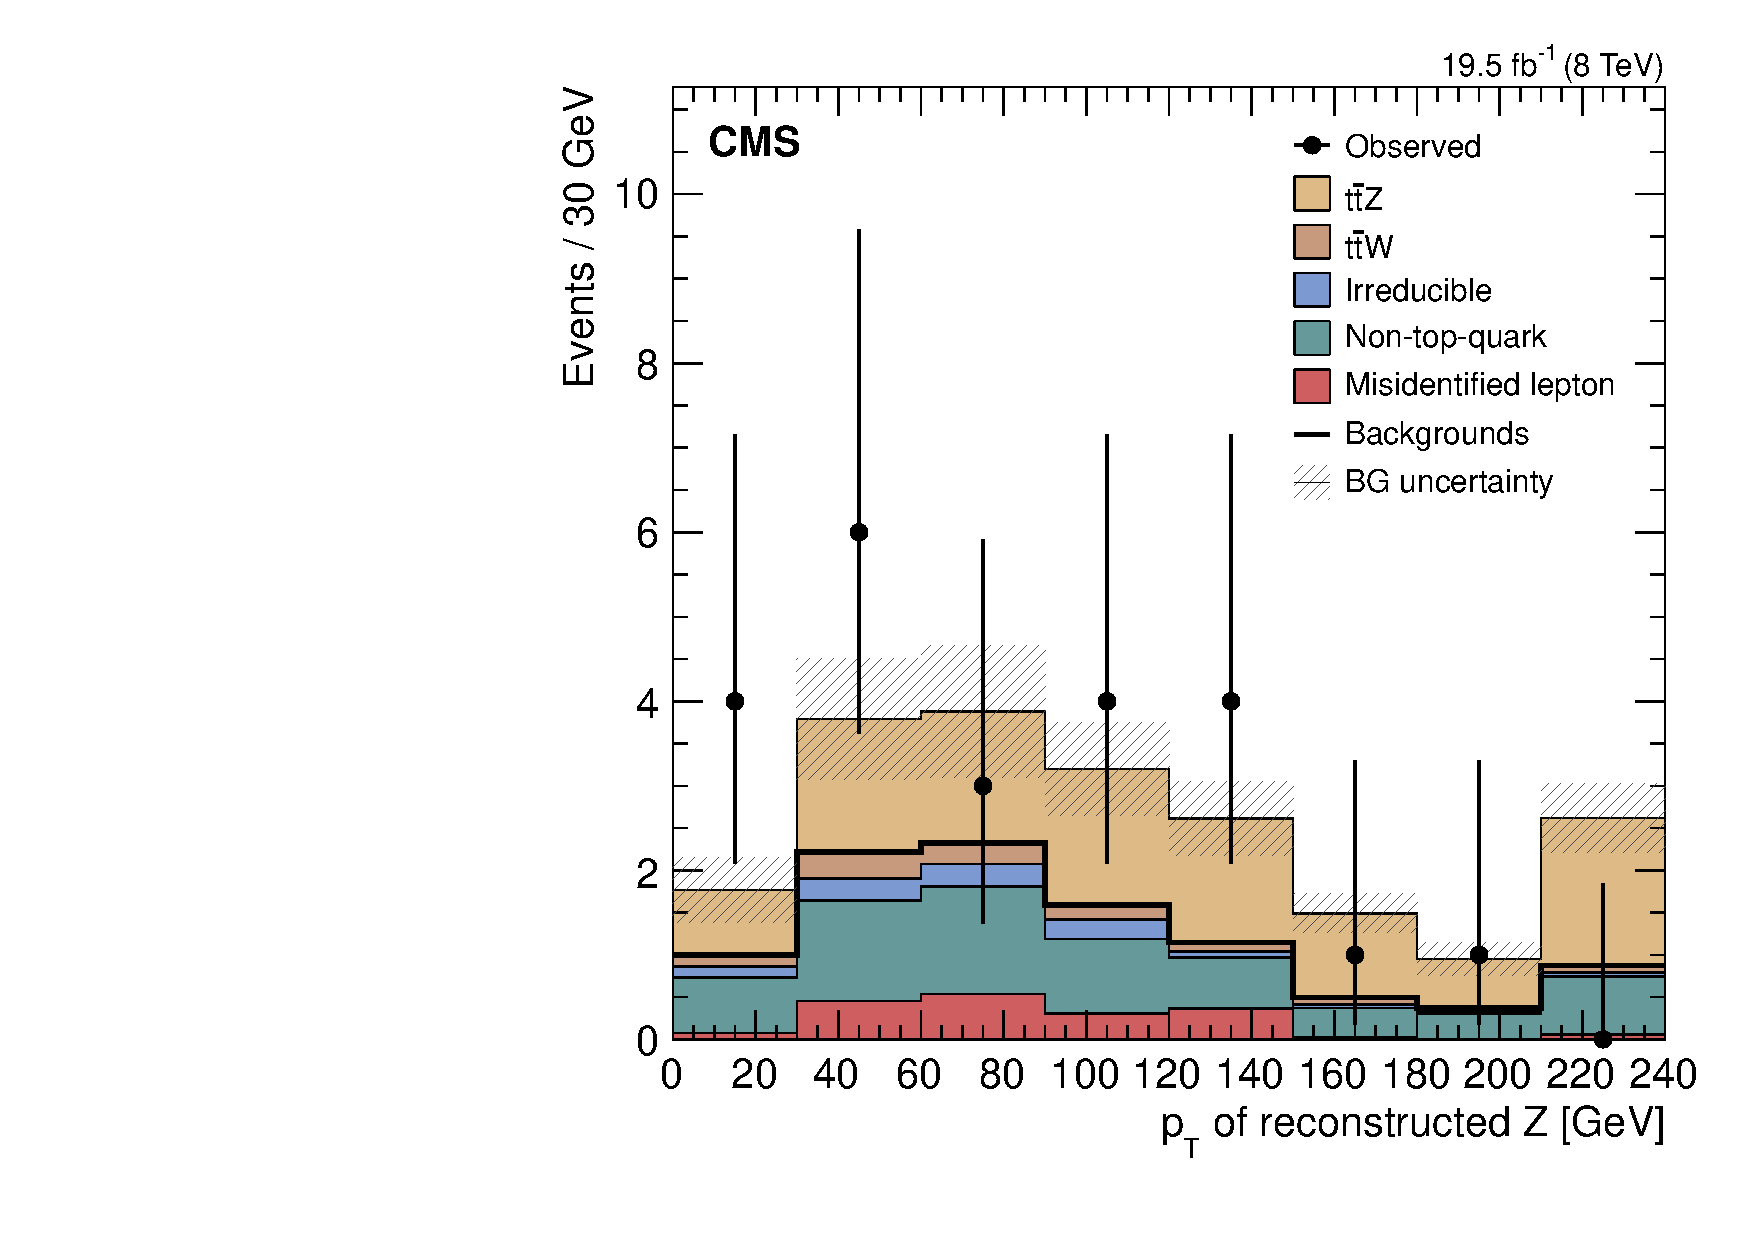
\includegraphics[width=0.48\linewidth]{Figs/Plots_PreSelections/hZPt_3L2b.pdf}
%\includegraphics[width=0.48\linewidth]{place_holders/index.png}
\caption{\label{fig:hzpt_3L2b}
\pt of the reconstructed Z boson after tri-lepton plus 2 b-Tag selections.
}
\end{center}
\end{figure}

\begin{figure}[h]
\begin{center}
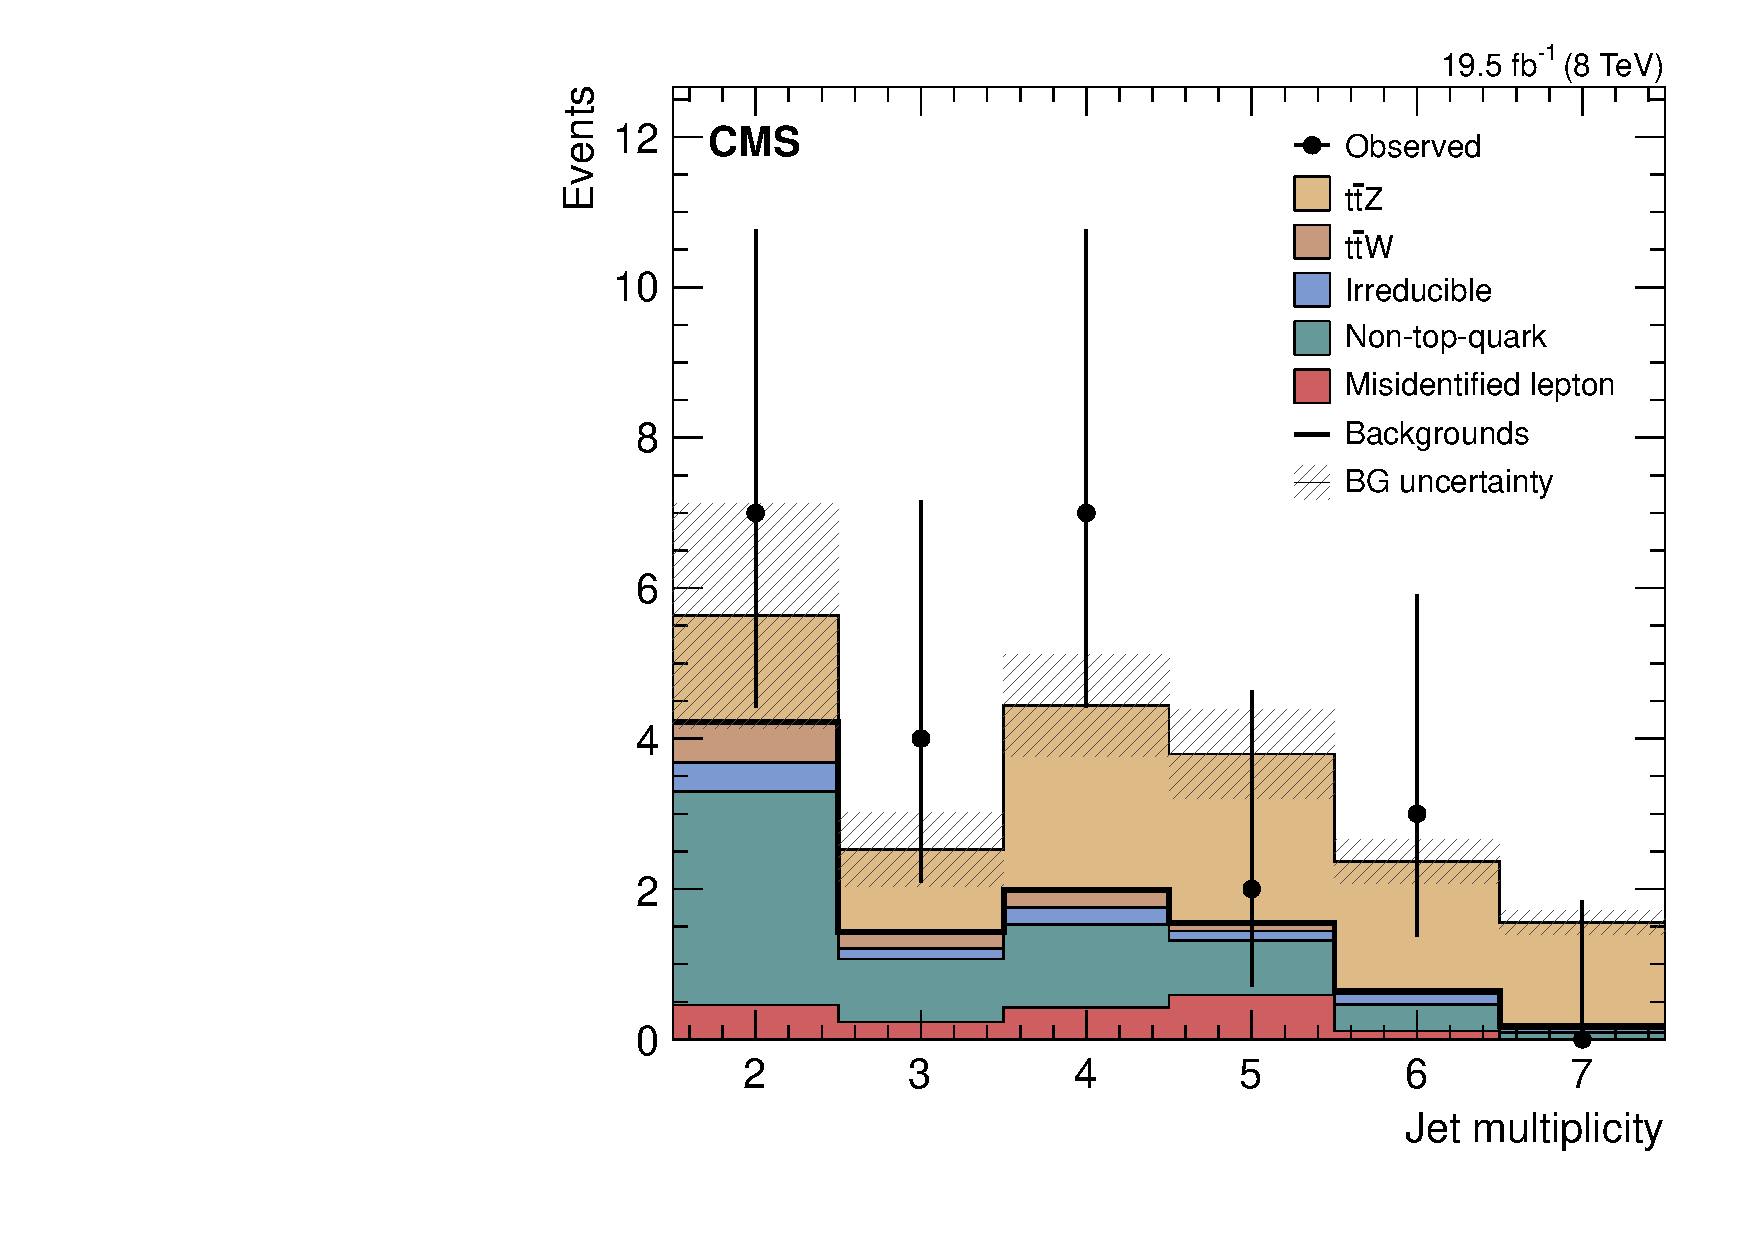
\includegraphics[width=0.48\linewidth]{Figs/Plots_PreSelections/hNJets_3L2b.pdf}
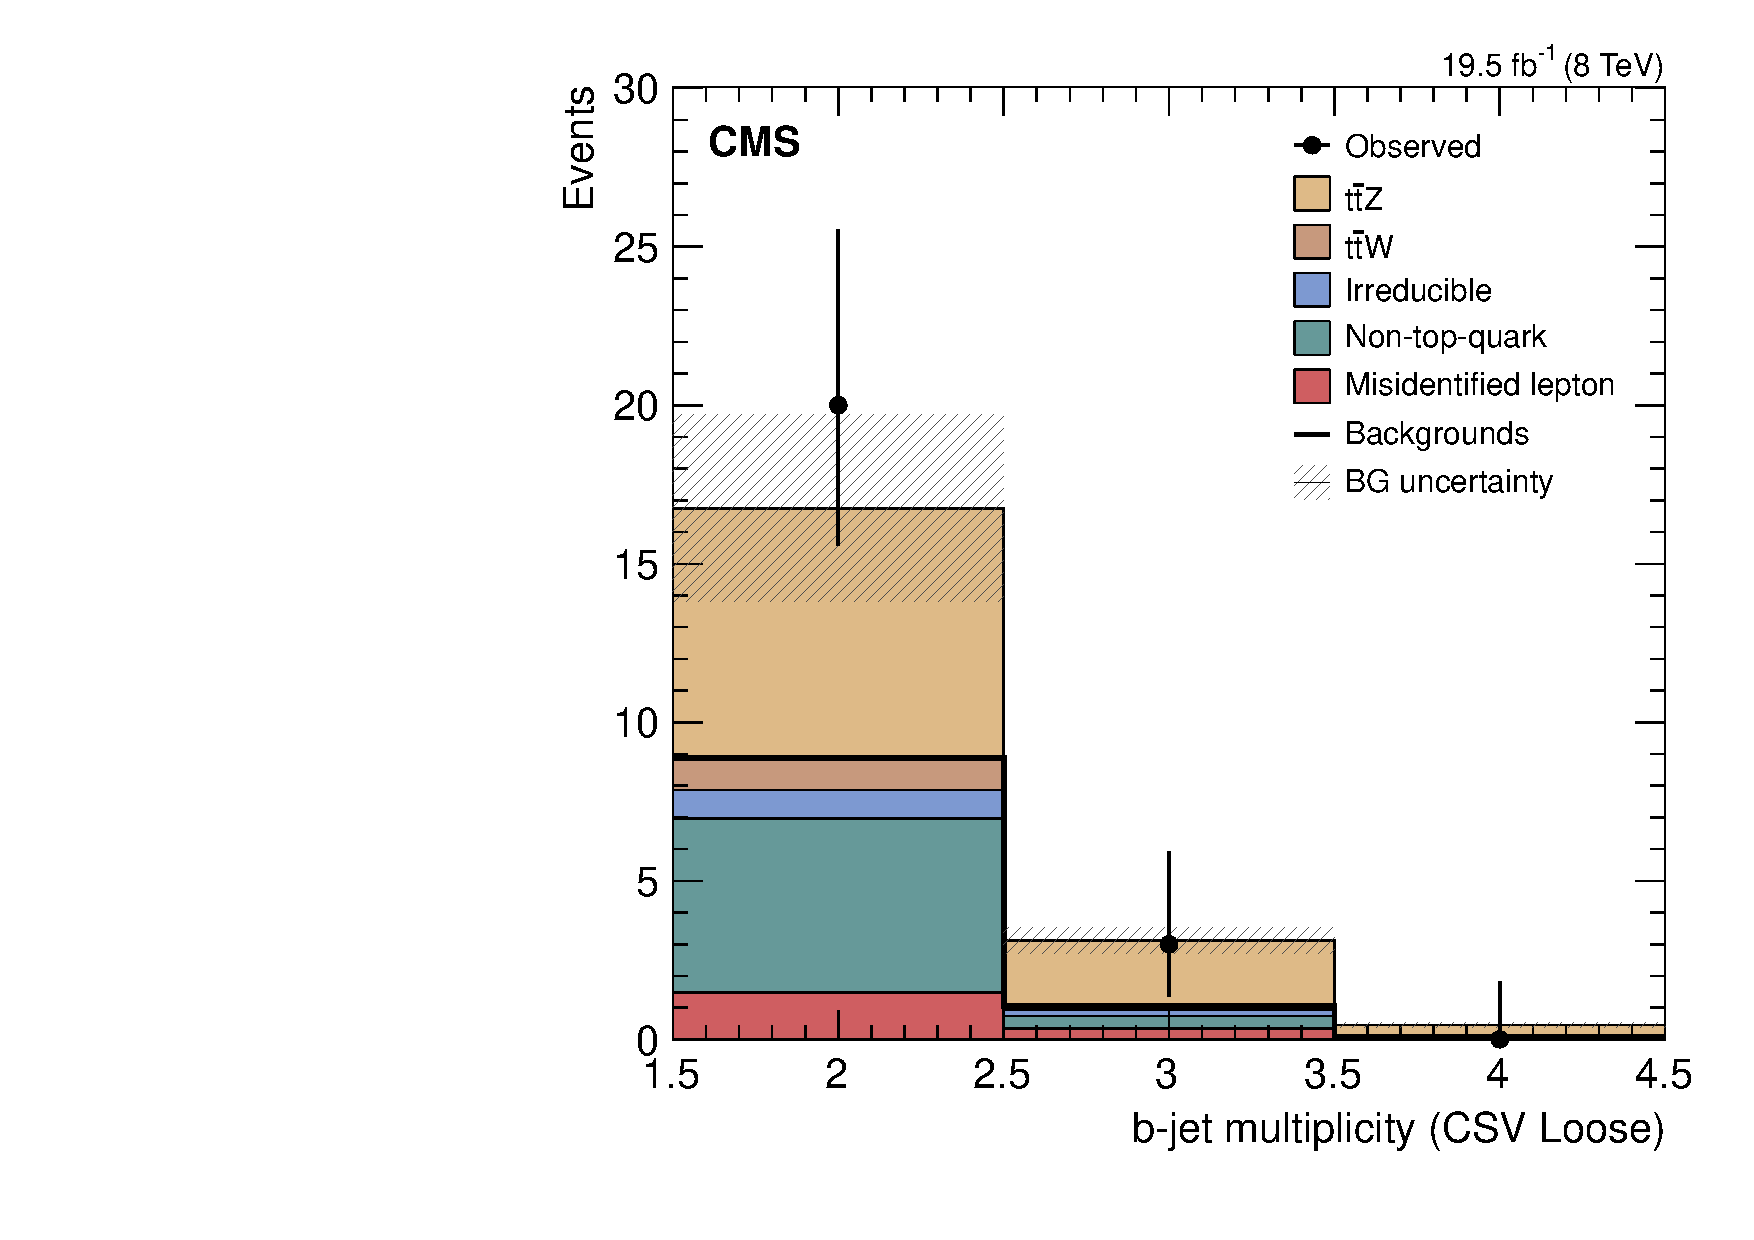
\includegraphics[width=0.48\linewidth]{Figs/Plots_PreSelections/hNLoose_3L2b.pdf}
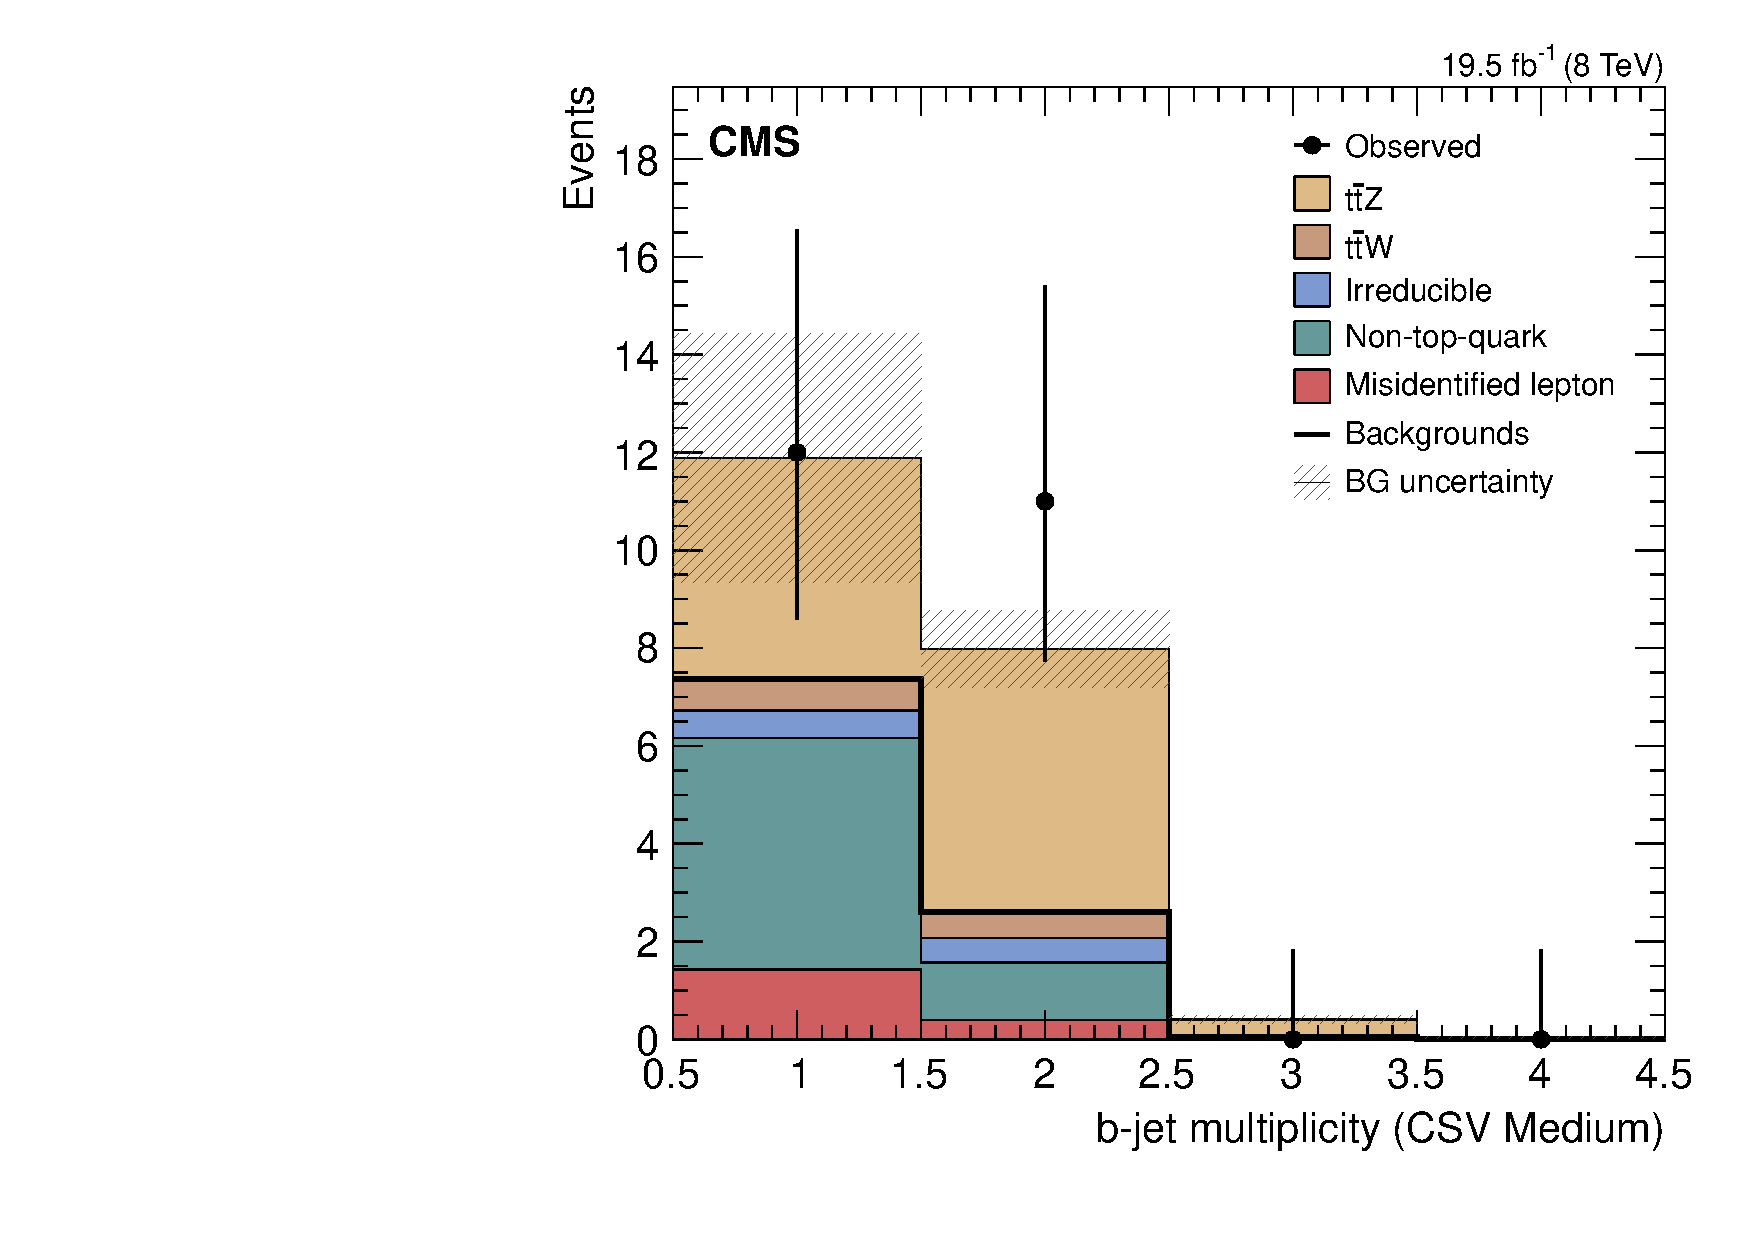
\includegraphics[width=0.48\linewidth]{Figs/Plots_PreSelections/hNMedium_3L2b.pdf}
\caption{\label{fig:jetmult_3L2b}
Jet Multiplicities. Left: Number of pfJets after tri-lepton plus 2 b-Tag selections. Middle: Number of CSVL b-Tags. Right: Number of CSVM b-Tags.
}
\end{center}
\end{figure}

\begin{figure}[h]
\begin{center}
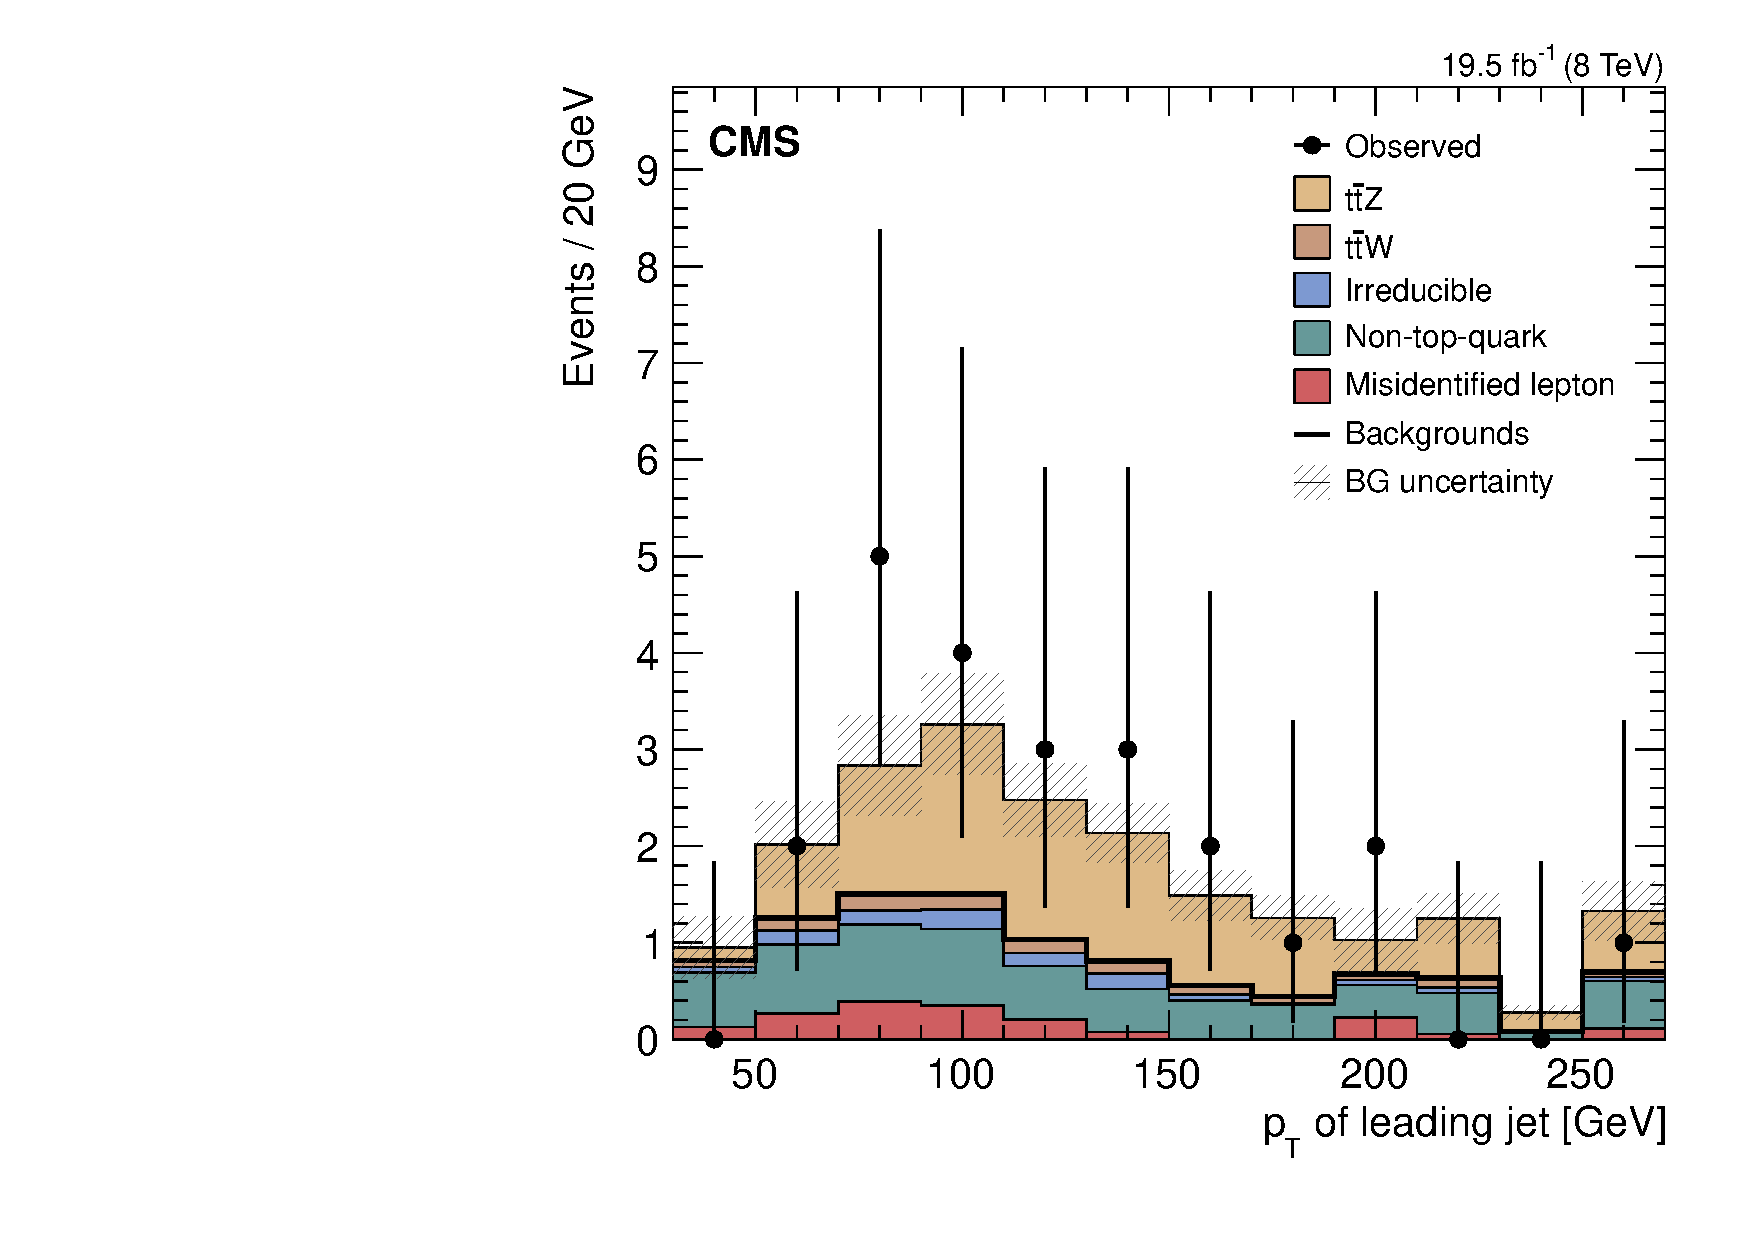
\includegraphics[width=0.48\linewidth]{Figs/Plots_PreSelections/hJ1Pt_3L2b.pdf}
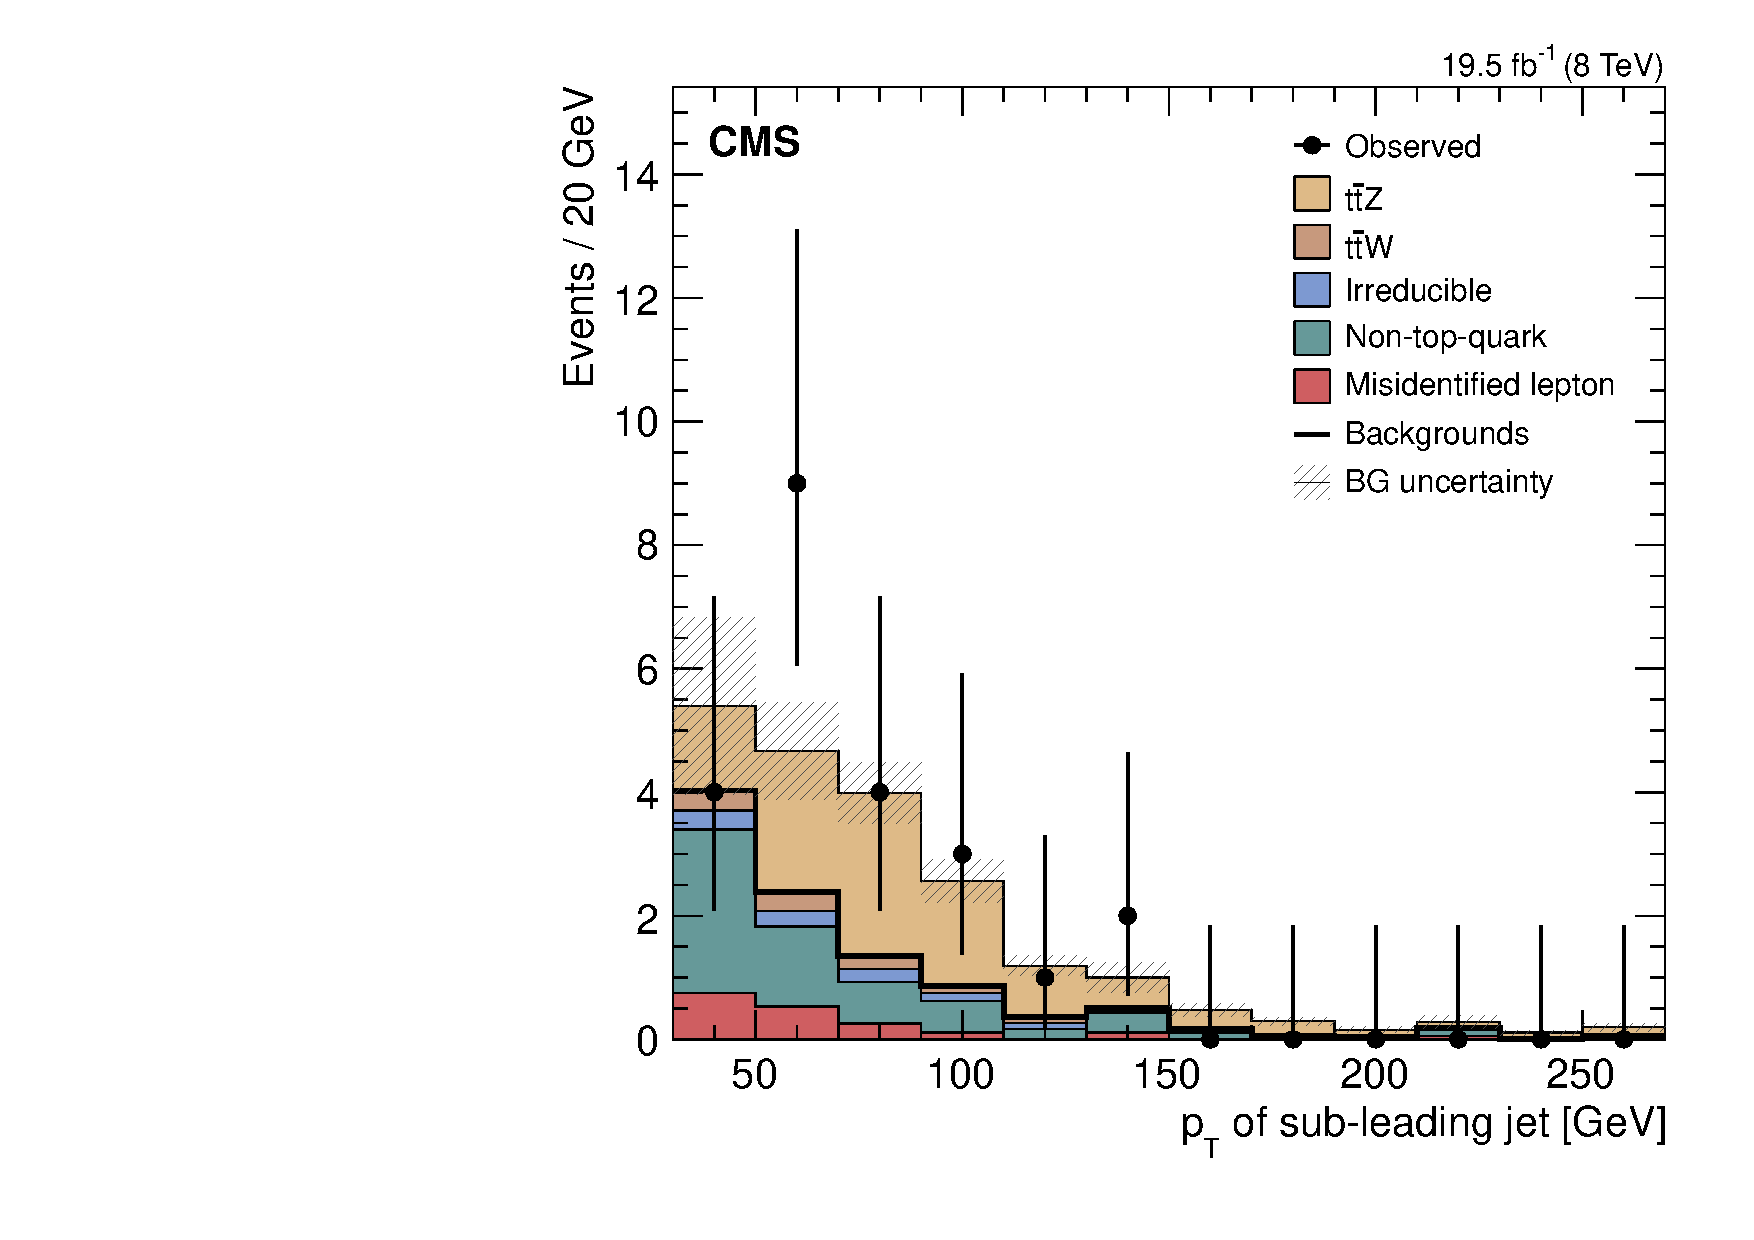
\includegraphics[width=0.48\linewidth]{Figs/Plots_PreSelections/hJ2Pt_3L2b.pdf}
\caption{\label{fig:JPt_3L2b}
Jet \pt . Left: \pt of leading jet after tri-lepton plus 2 b-Tag selections. Right: \pt of sub leading jet after tri-lepton plus 2 b-Tag selections.
}
\end{center}
\end{figure}

\begin{figure}[h]
\begin{center}
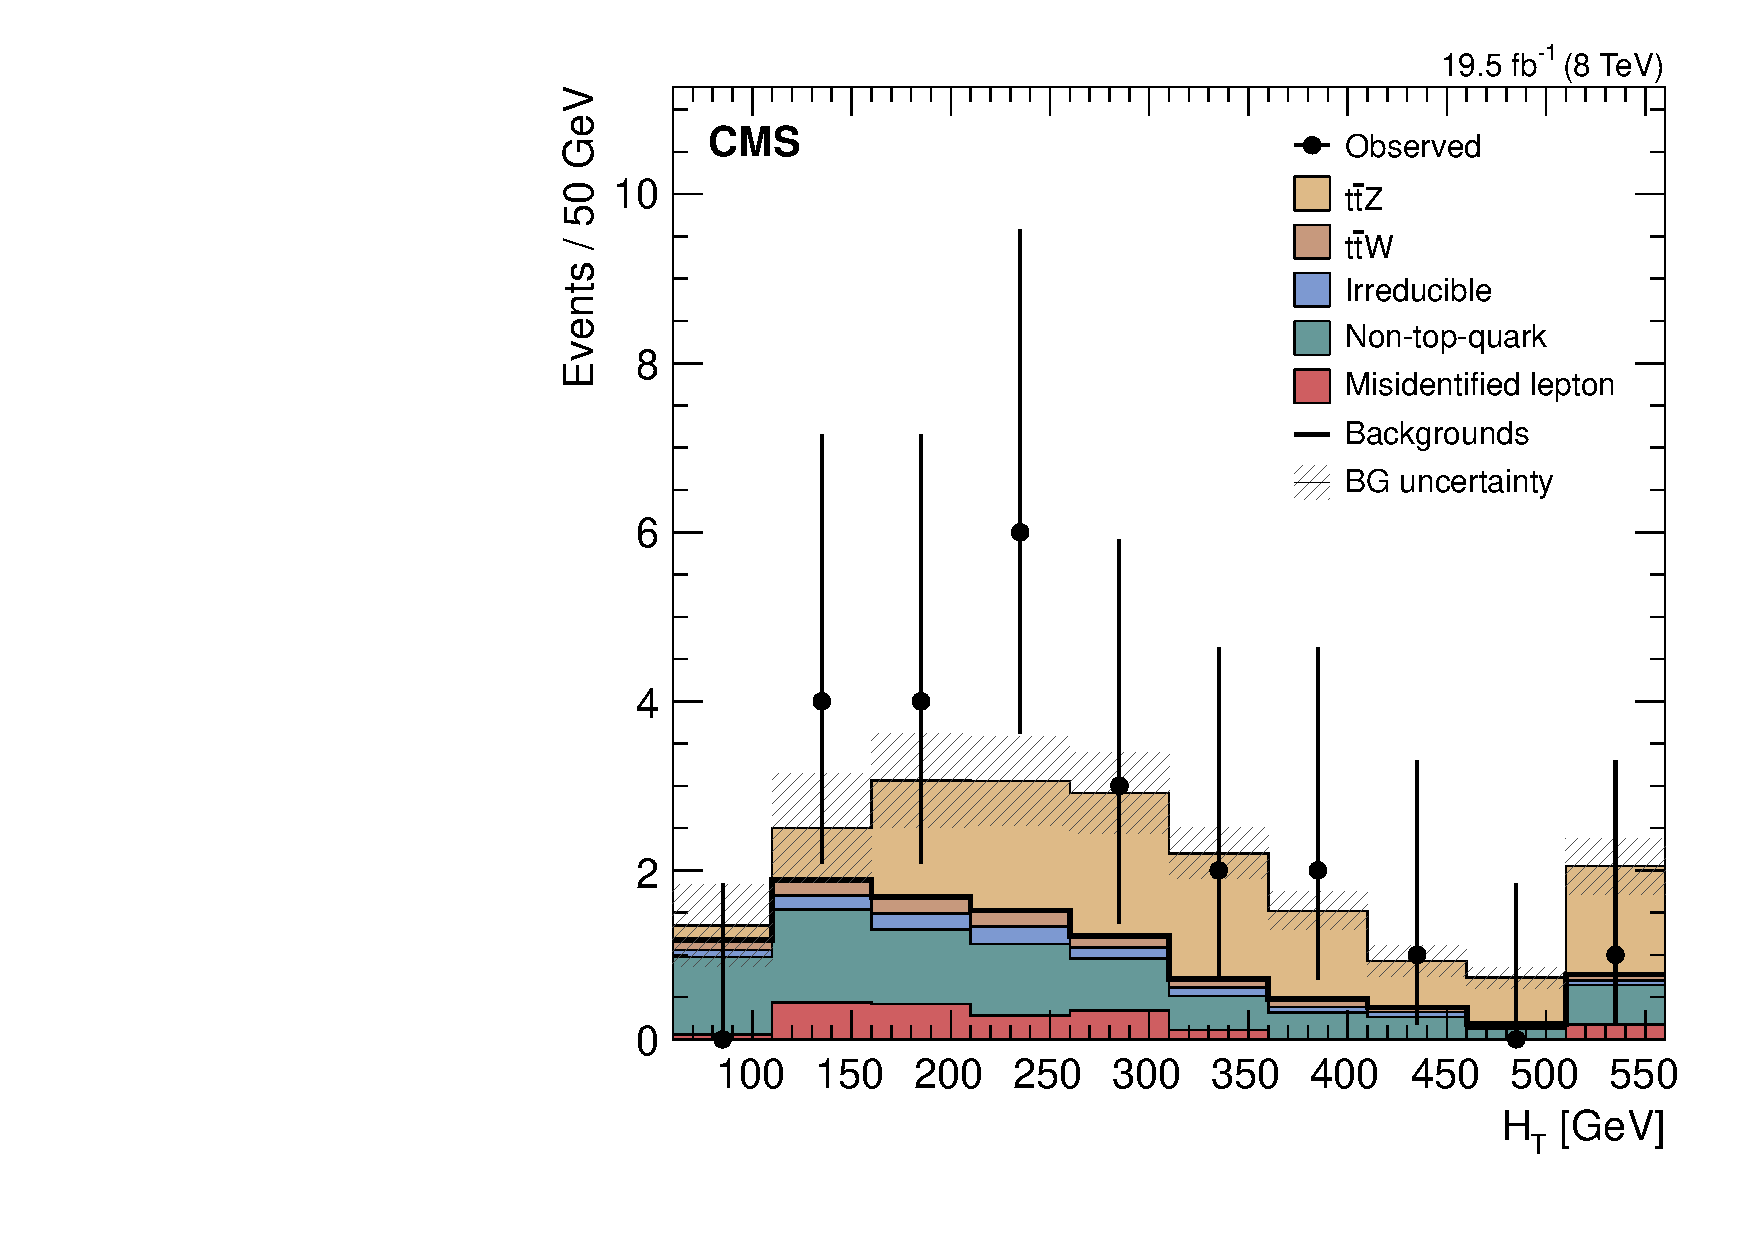
\includegraphics[width=0.48\linewidth]{Figs/Plots_PreSelections/hHt_3L2b.pdf}
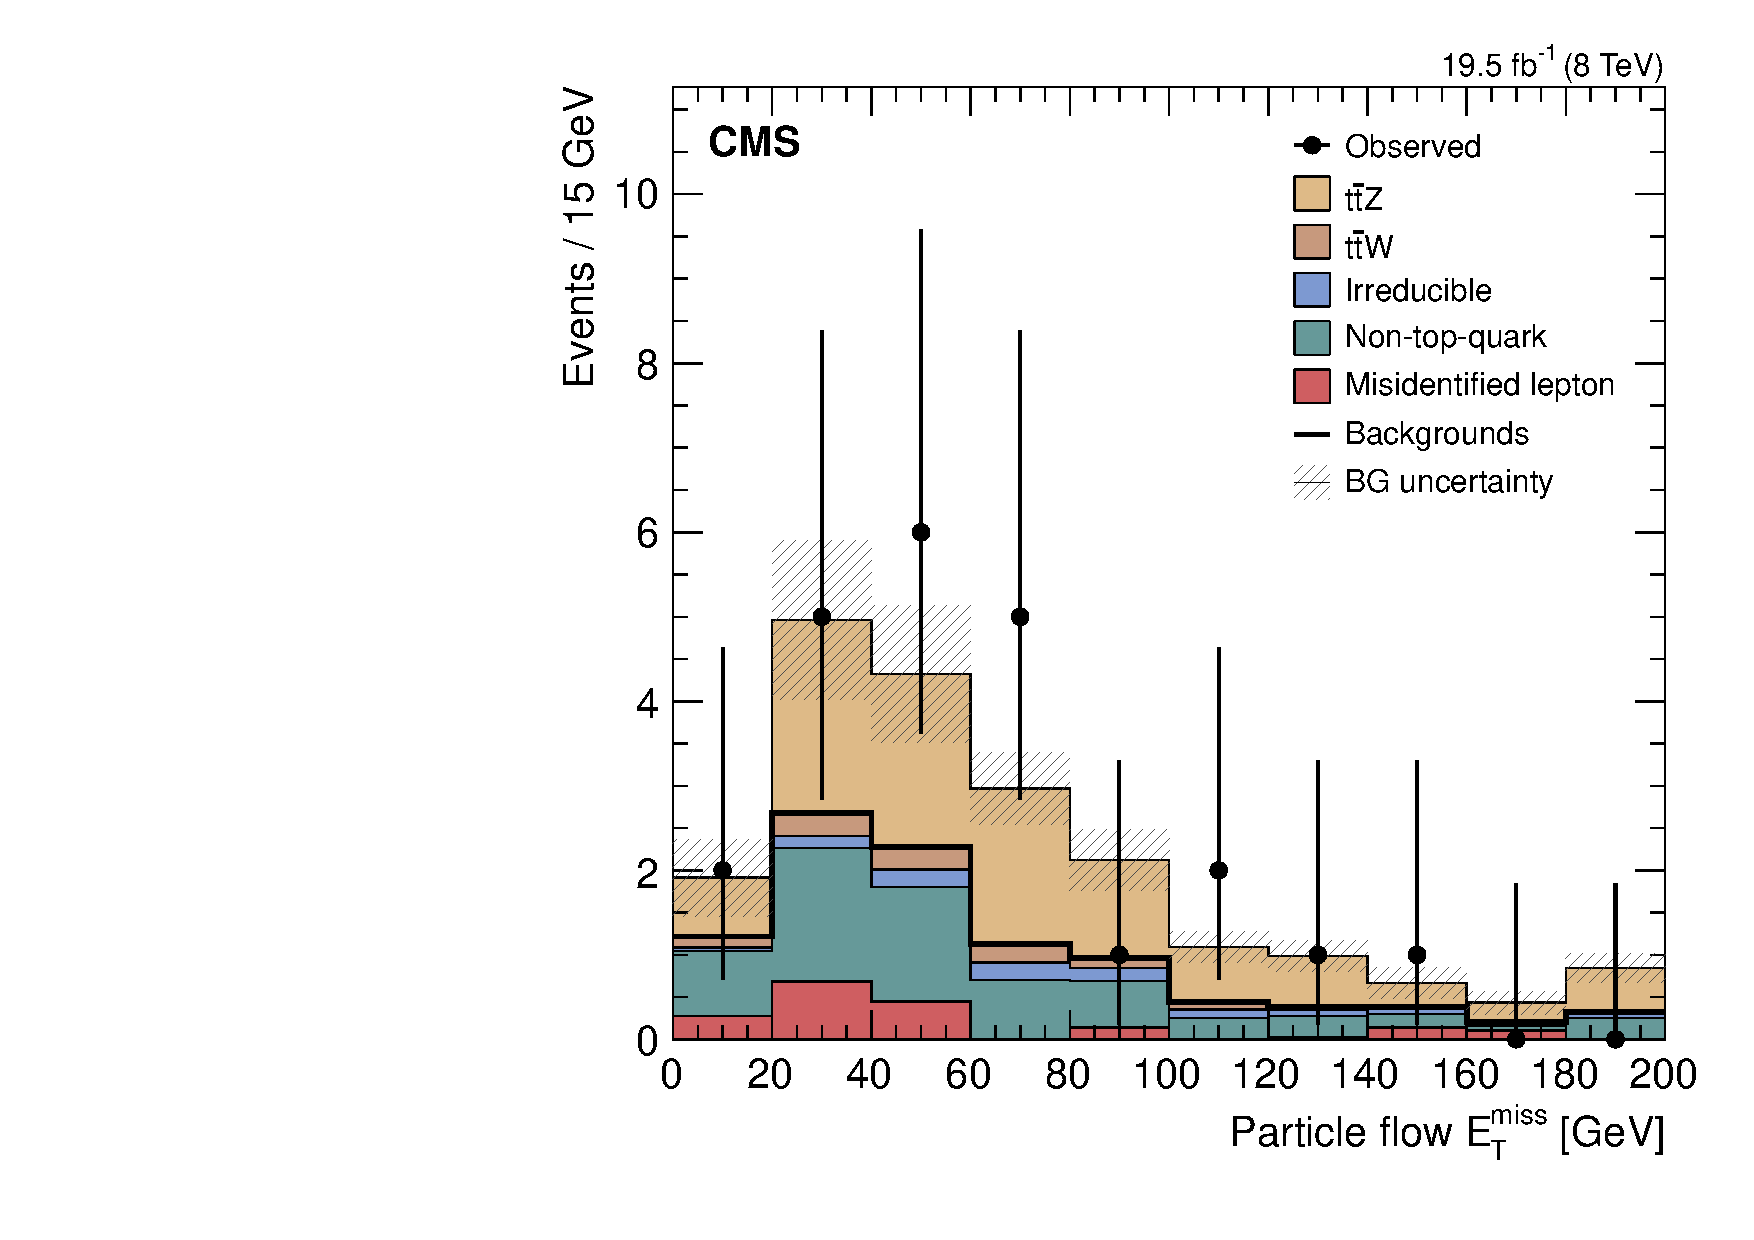
\includegraphics[width=0.48\linewidth]{Figs/Plots_PreSelections/hPFMet_3L2b.pdf}
\caption{\label{fig:hht_pfmet_3l}
Ht (Left) and pfMet (Right) after tri-lepton plus 2 b-Tag selections.
}
\end{center}
\end{figure}







         
	\section{yields}
	The yields in data and MC are summarized in Table ~\ref{tab:yields} after applying the full analysis selections as listed in Section ~\ref{sec:eventsel}. The MC is normalized to \intLumi of luminosity to match the data, and scaled by the lepton efficiency scale factors and b-Tag discriminant re-weighting as described in Sections ~\ref{sec:tagnprobe} and ~\ref{sec:discReshape} respectively. The data yields are shown along side the MC yields to help demonstrate the relative contributions of the individual backgrounds. The data driven backgrounds were shown in the previous sections and will be used in the next section to calculate the \ttZ \ signal. The irreducible backgrounds will be estimated from the yields in this table using the line labeled $t\overline{t}$X/tbZ/VZZ. Given our lack of knowledge of cross sections for these processes and an inability to validate these MC samples against data, we assign a 50\% systematic.

\begin{table}[ht!]
\begin{center}
\caption{\small \label{tab:yields} Data and pure MC yields after full analysis selections with \intLumi.}
\begin{tabular}{c|ccccc}\hline
&Yields (All)&Yields ($\mu\mu\mu$)&Yields ($\mu\mu$e)&Yields (ee$\mu$)&Yields (eee)\\
\hline \hline
W $\rightarrow \ell \nu$ & 0.00$\pm$0.89 & 0.00$\pm$0.89 & 0.00$\pm$0.89 & 0.00$\pm$0.89 & 0.00$\pm$0.89\\
VV $\rightarrow 2 \ell$ & 0.04$\pm$0.07 & 0.02$\pm$0.06 & 0.02$\pm$0.06 & 0.00$\pm$0.06 & 0.00$\pm$0.06\\
$t\overline{t}$ & 0.32$\pm$0.12 & 0.11$\pm$0.08 & 0.14$\pm$0.10 & 0.04$\pm$0.09 & 0.03$\pm$0.09\\
DY $\rightarrow 2 \ell$  & 0.00$\pm$0.60 & 0.00$\pm$0.60 & 0.00$\pm$0.60 & 0.00$\pm$0.60 & 0.00$\pm$0.60\\
VZ $\rightarrow 3\ell$ or $4\ell$ & 1.02$\pm$0.09 & 0.25$\pm$0.04 & 0.34$\pm$0.05 & 0.19$\pm$0.04 & 0.23$\pm$0.04\\
WWV & 0.13$\pm$0.03 & 0.03$\pm$0.01 & 0.02$\pm$0.01 & 0.05$\pm$0.02 & 0.03$\pm$0.01\\
\ttX/tbZ/VZZ & 0.98$\pm$0.08 & 0.32$\pm$0.05 & 0.20$\pm$0.04 & 0.24$\pm$0.05 & 0.22$\pm$0.04\\
\ttZ & 8.15$\pm$0.38 & 2.45$\pm$0.21 & 2.09$\pm$0.19 & 1.99$\pm$0.19 & 1.62$\pm$0.17\\
\hline \hline
Total Bkg MC (19.5 fb$^{-1}$) & 2.49$\pm$1.09 & 0.74$\pm$1.08 & 0.72$\pm$1.08 & 0.51$\pm$1.08 & 0.52$\pm$1.08\\
\hline
Total Sig+Bkg MC (19.5 fb$^{-1}$) & 10.64$\pm$1.15 & 3.19$\pm$1.10 & 2.81$\pm$1.10 & 2.50$\pm$1.10 & 2.14$\pm$1.09\\
\hline
Data (19.5 fb$^{-1}$) & 12.$\pm$3.46 & 3.$\pm$1.73 & 2.$\pm$1.41 & 4.$\pm$2.00 & 3.$\pm$1.73\\
\hline
\end{tabular}
\end{center}
\end{table}



	\section{Measured Signal and Background Subtraction}
Compiling the information in the preceding sections, an estimate can be made for the \ttZ \ signal in the measured data. The contribution due to di-lepton final states that pass the selection due to an additional ``fake" lepton in the event is described in Section ~\ref{sec:fakerate} and the contribution from tri-lepton events that pass the selection due to b-Tagged jets that arise from gluon radiation is described in Section ~\ref{sec:brate}. Finally, the irreducible backgrounds which cannot be estimated by a data driven method are taken from the row labeled ``\ttX/tbZ/VZZ" in Table ~\ref{tab:yields} where the ``X" is short hand for W, $\gamma$, or WW. Table ~\ref{tab:signal_minus_bkg} summarizes the full yields in data after selections as well as the background estimates. Additionally a final estimate for the \ttZ \ to 3 lepton signal is shown.

\begin{table}[ht!]
\begin{center}
\caption{\small \label{tab:signal_minus_bkg} Data and pure MC yields after full analysis selections with \intLumi.}
\begin{tabular}{c|c}\hline
 & Measurement\\
\hline \hline
Data (19.5 fb $^{-1}$)                         & $12. $ \\
%\hdashline
Bkg from Non-Prompt Leptons                   &  $- 1.13 \pm 0.51_{st} \pm 0.57_{sy}$ \\
Bkg from b-Tags From Radiation                &  $- 2.27 \pm 0.51_{st} \pm 1.14_{sy}$ \\
Bkg from Irreducible                          &  $- 0.98 \pm 0.08_{st} \pm 0.49_{sy}$ \\
%\hdashline
Total Background Prediction                   &  $-4.38 \pm 0.73_{bkg st} \pm 1.37_{bkg sy}$ \\
\hline
Predicted Signal                              &  $7.62 \pm 3.46_{data st} \pm 0.73_{bkg st} \pm 1.37_{bkg sy}$ \\	
\hline
\end{tabular}
\end{center}
\end{table}



	
	\subsection{top mass reconstruction}
	A simple algorithm is chosen to identify the jets from the hadronic top. There are few events, the algorithm must choose jets for each one, yet be simple enough not to sculpt the distribution. We following steps are taken:
\begin{enumerate}
\item Choose 3 jets, one of which has a CSVL or better b-tag that minimizes 3 jet system $\Delta R$ defined as \\
$\Delta R_{j1,j2,b1} = \sqrt{ (\Delta R_{j1, ``top"}) ^2 + (\Delta R_{j2, ``top"}) ^2 + (\Delta R_{b1, ``top"}) ^2 }$\\
where ``top'' is the composite object created by summing the 4-vectors of the 3 jets.
\item Choose the highest pt b-Jet out of the remaining b-Tagged jets that are not part of the 3 jet system in step 1. This b-jet is considered to be from the leptonic top.
\end{enumerate}

Figure ~\ref{fig:htopmass_3l2j2b} shows the hadronic top mass, hadronic W mass, and invariant mass of the b-Jet and lepton from the leptonic top (with the neutrino unaccounted for for obvious reasons).


\begin{figure}[h]
\begin{center}
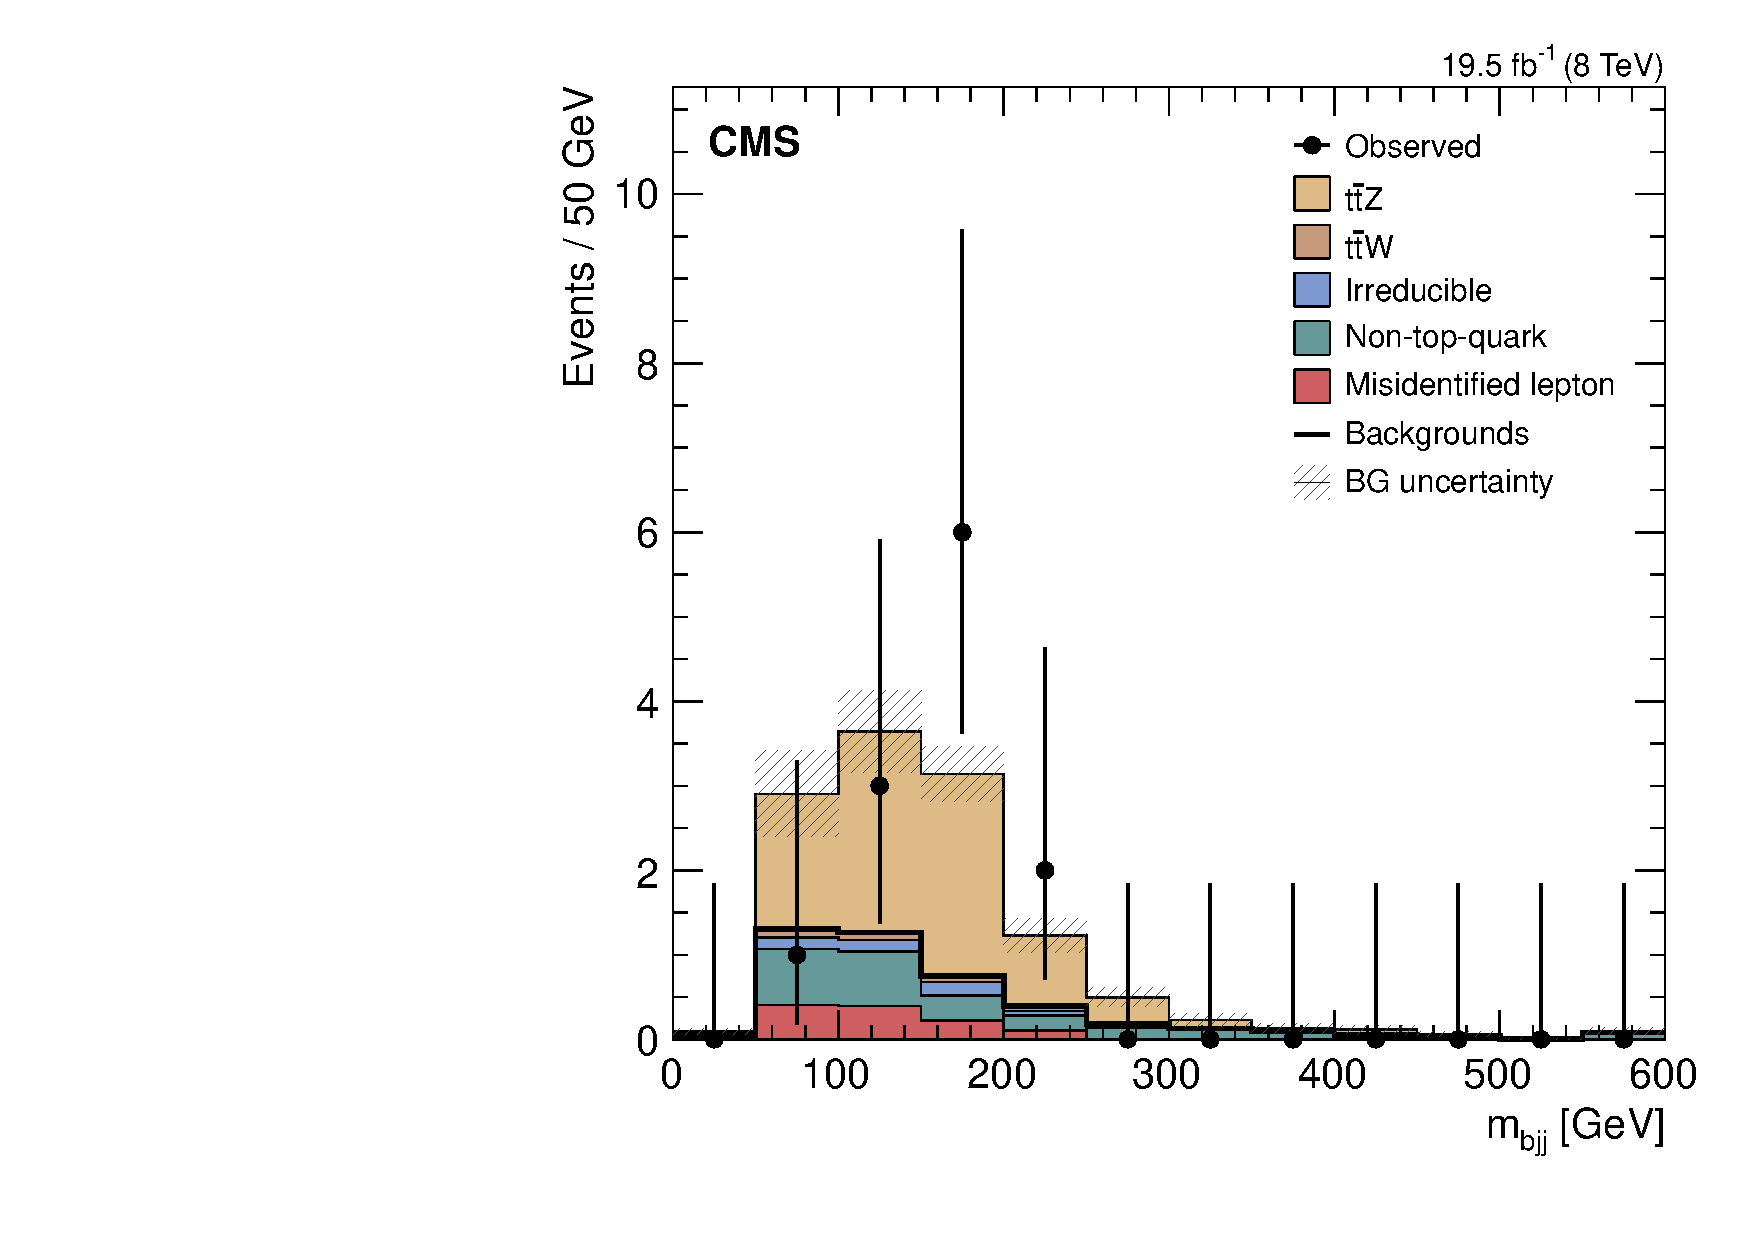
\includegraphics[width=0.48\linewidth]{Figs/Plots_Final_Selections/hTopMass_3L2J2b.pdf}
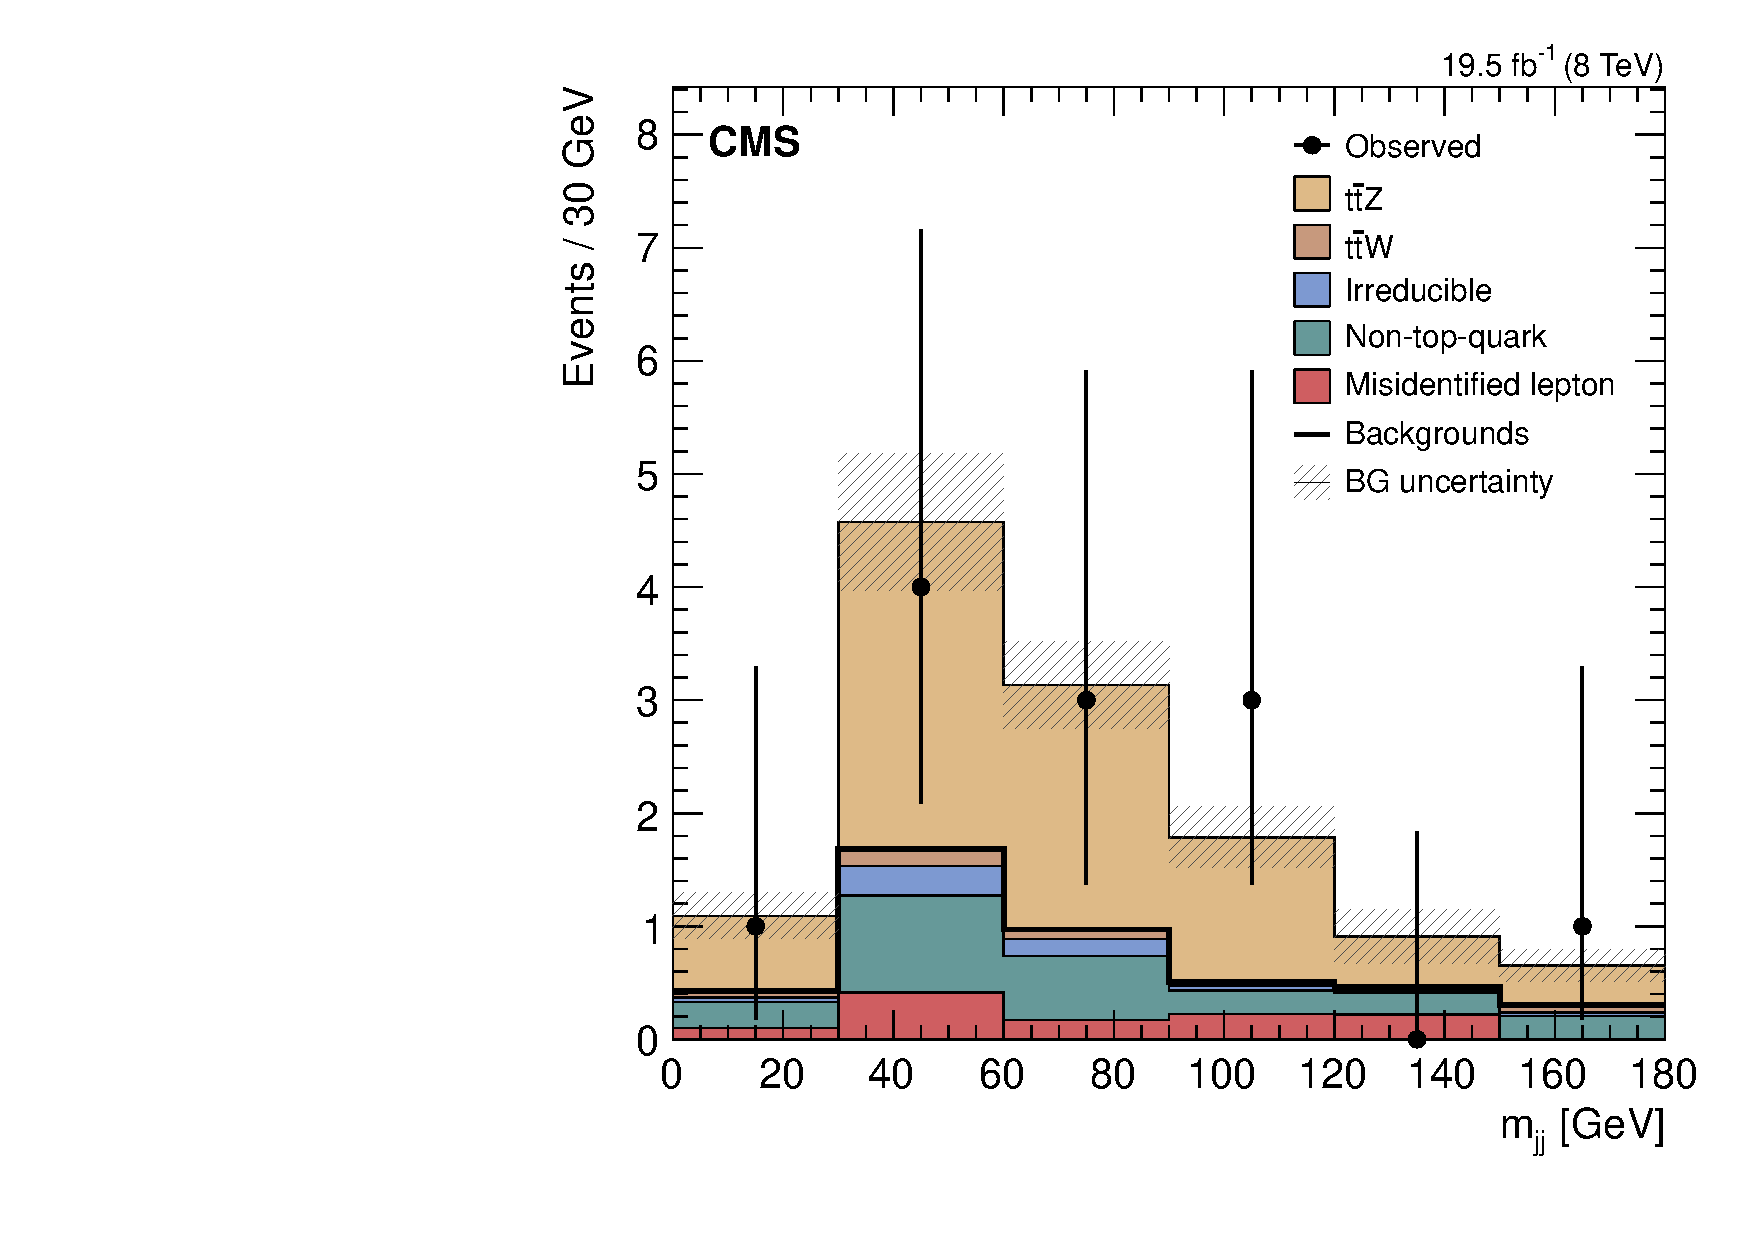
\includegraphics[width=0.48\linewidth]{Figs/Plots_Final_Selections/hTopWMass_3L2J2b.pdf}
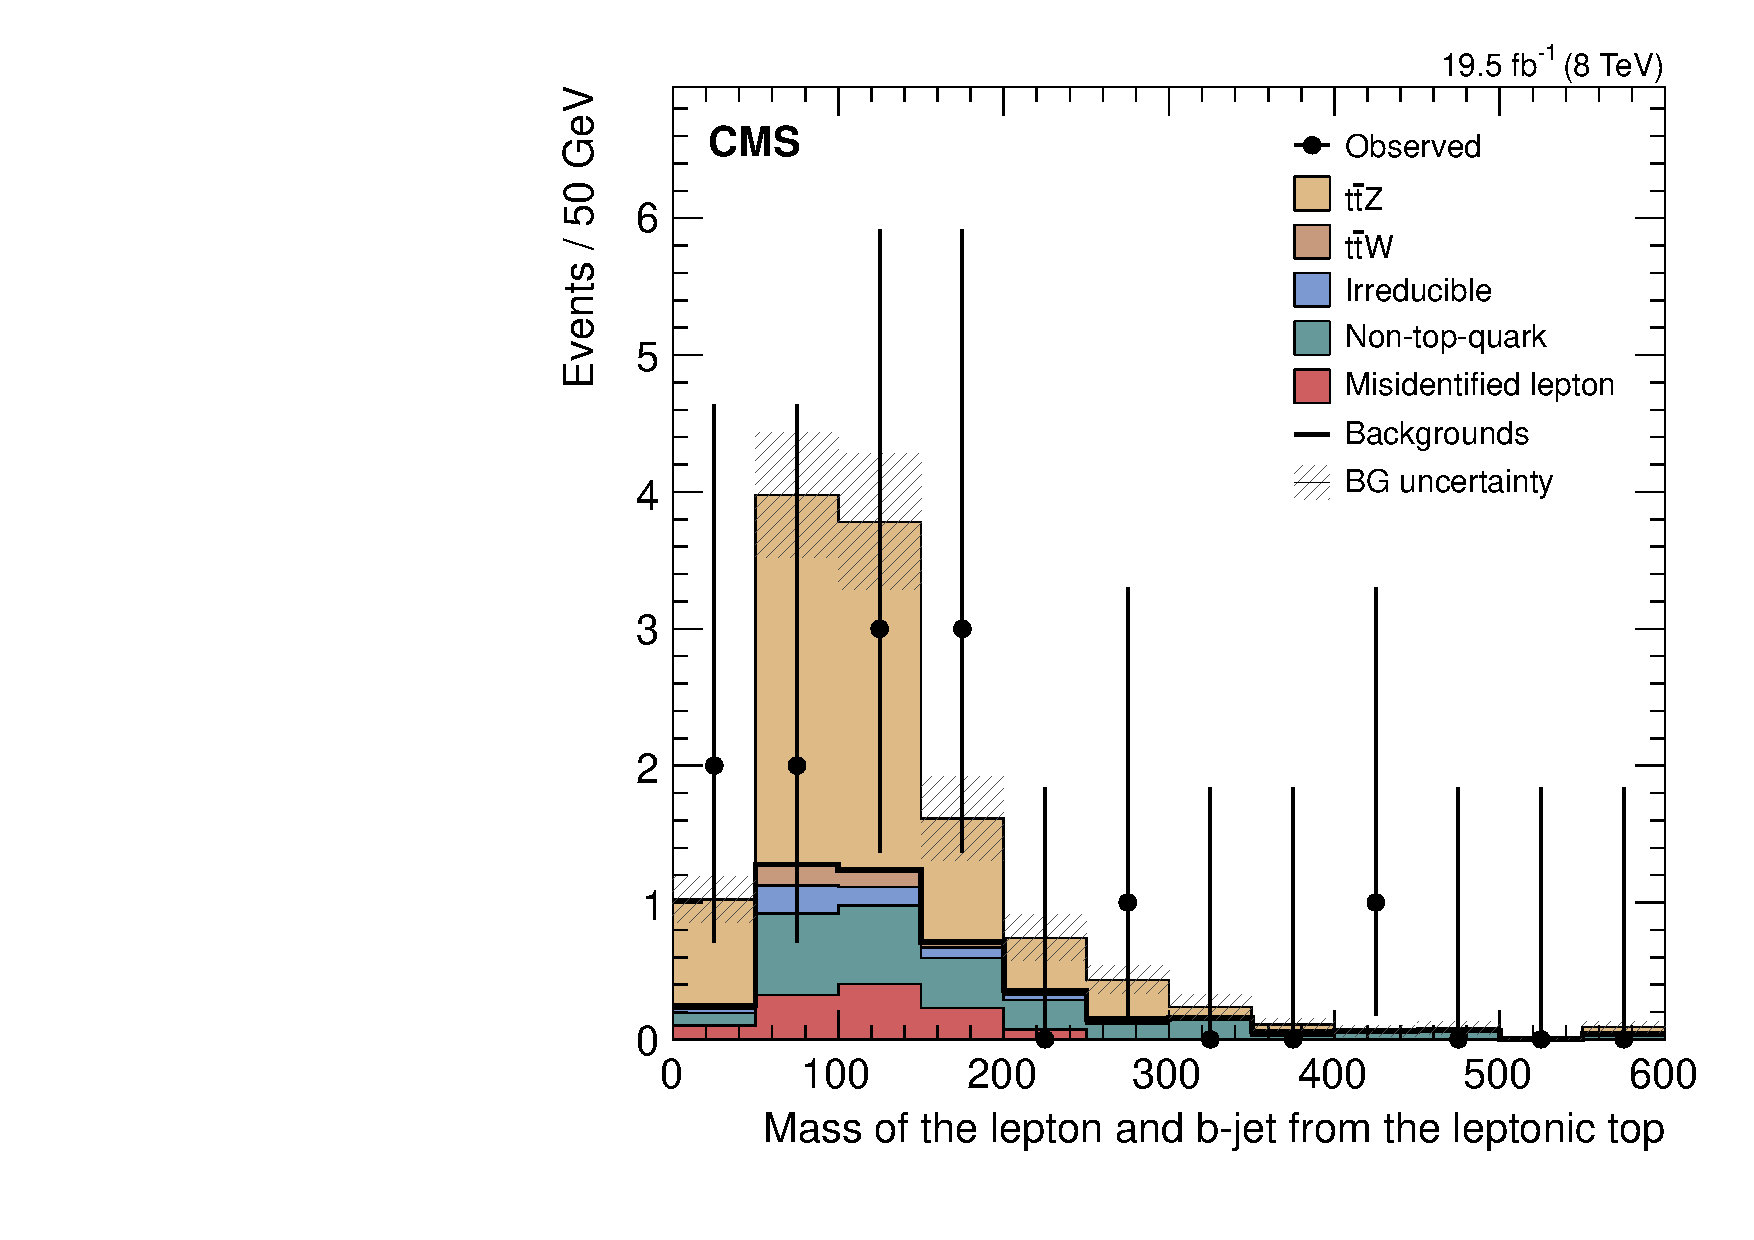
\includegraphics[width=0.48\linewidth]{Figs/Plots_Final_Selections/hTopbLMass_3L2J2b.pdf}
\caption{\label{fig:htopmass_3l2j2b}
Reconstructed mass of the hadronic top is shown after all selections have been applied (Top Left). Reconstructed mass of the hadronic W is shown after all selections have been applied(Top Right). Invariant mass of the W lepton with the b-Jet from the leptonic top is shown (Bottom).
}
\end{center}
\end{figure}
	
	
	
	
	
	
	
	\subsection{Distributions with full selections}
	REPLACE WHAT I CAN WITH PLOTS FROM THE FINAL PAPER\\
	
	
	The full analysis selection is described in Section ~\ref{sec:eventsel}. This includes leptonic selections of reconstructing a Z from two leptons and requiring a third lepton that could be from a W. It also includes requiring 4 or more jets with 2 of them being b-Tagged (one CSVL and one CSVM). After selection the \ttZ \ contribution as predicted in MC is strong and the backgrounds have been reduced to a manageable level. In the following plots, data driven predictions are again used for normalization of backgrounds while MC is used for the shape (except in the case of the irreducible backgrounds where MC is used for shape and normalization). Although being lower in statistics, there is reasonable agreement between data and predictions (shape and size). Relevant plots are shown below. Figure ~\ref{fig:hmass_3l2j2b} shows the reconstructed masses of the Z and the leptonic W (using \Mt) %while FIgure ~\ref{fig:htopmass_3l2j2b} shows the top (using the W \Mt \ for the W's contribution). 
These plots are used to demonstrate a degree of certainty that the correct events are being identified. %since the various underlying bosons and quarks can be reconstructed. \\

\begin{figure}[h]
\begin{center}
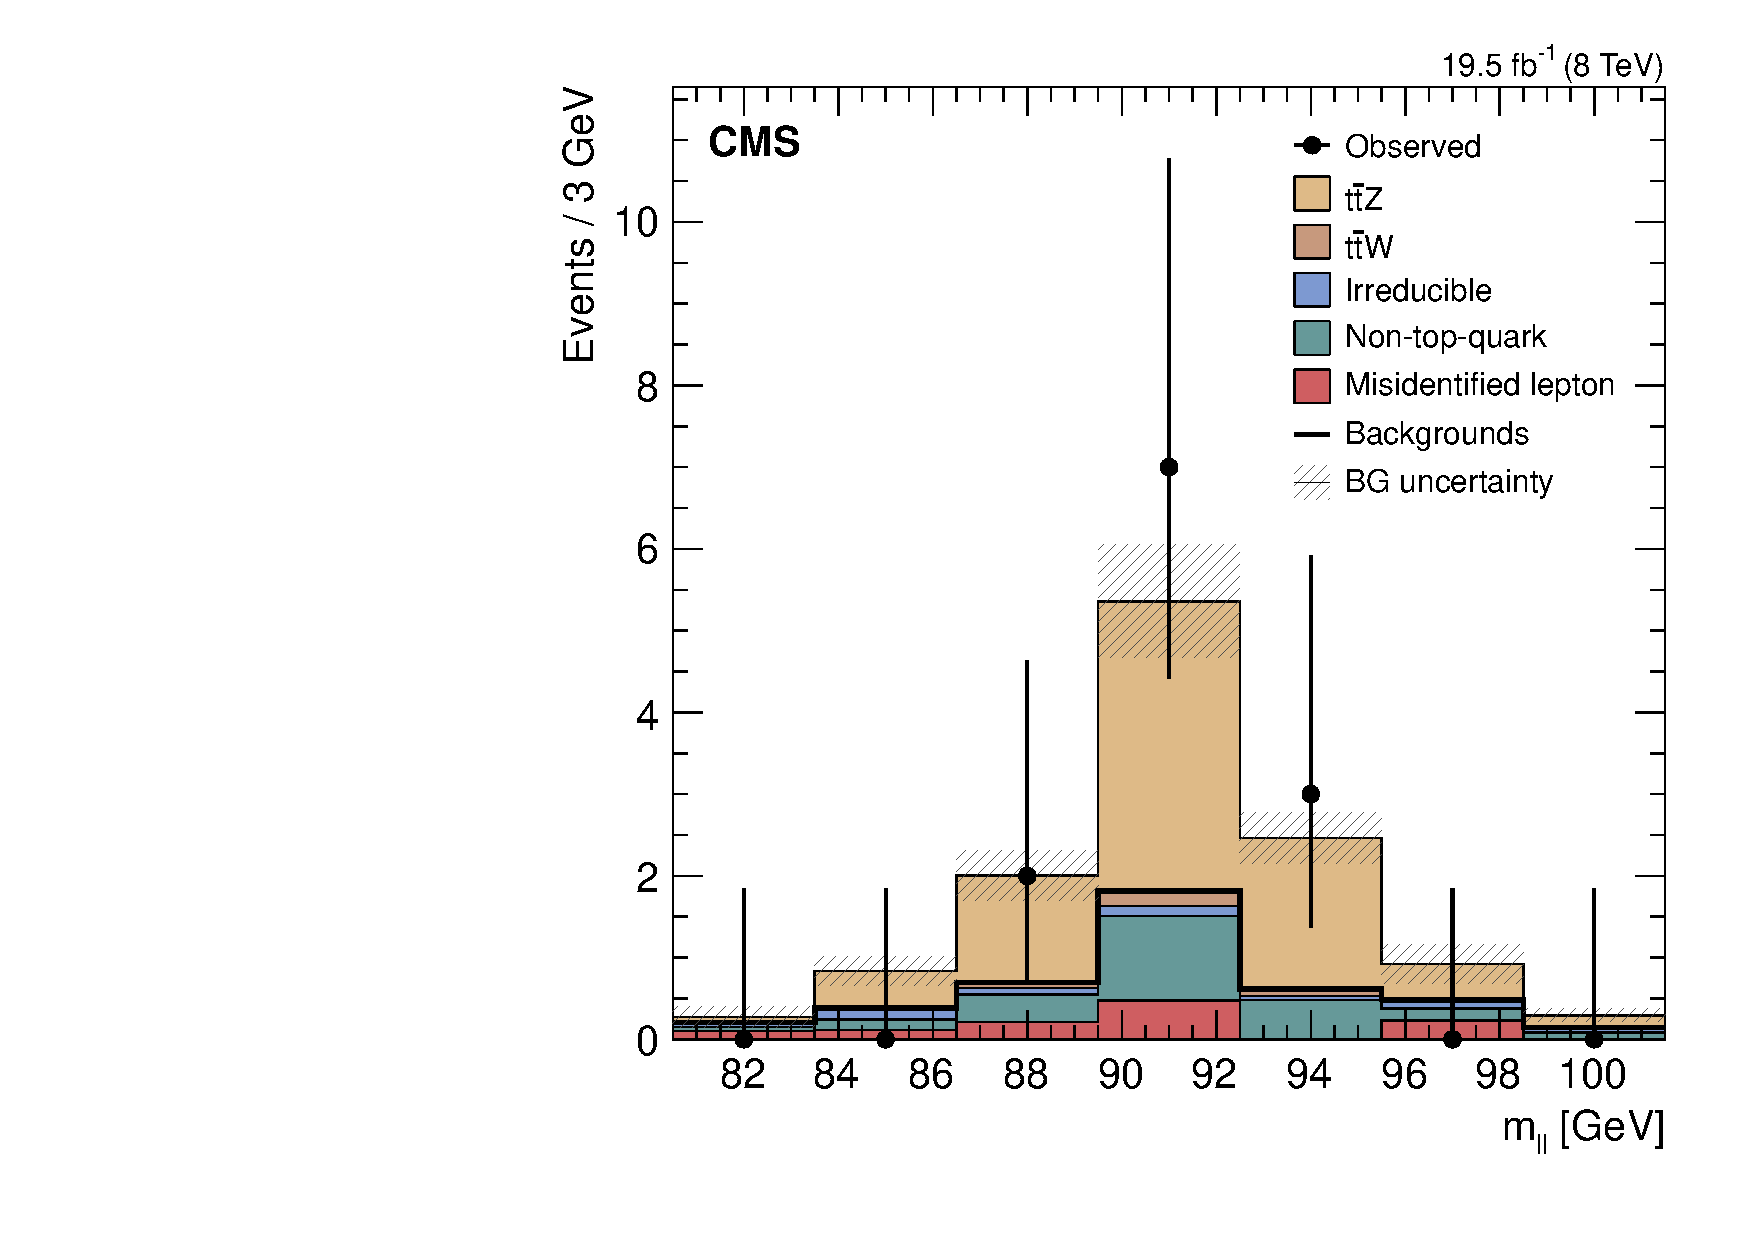
\includegraphics[width=0.48\linewidth]{Figs/Plots_Final_Selections/hZMass_3L2J2b.pdf}
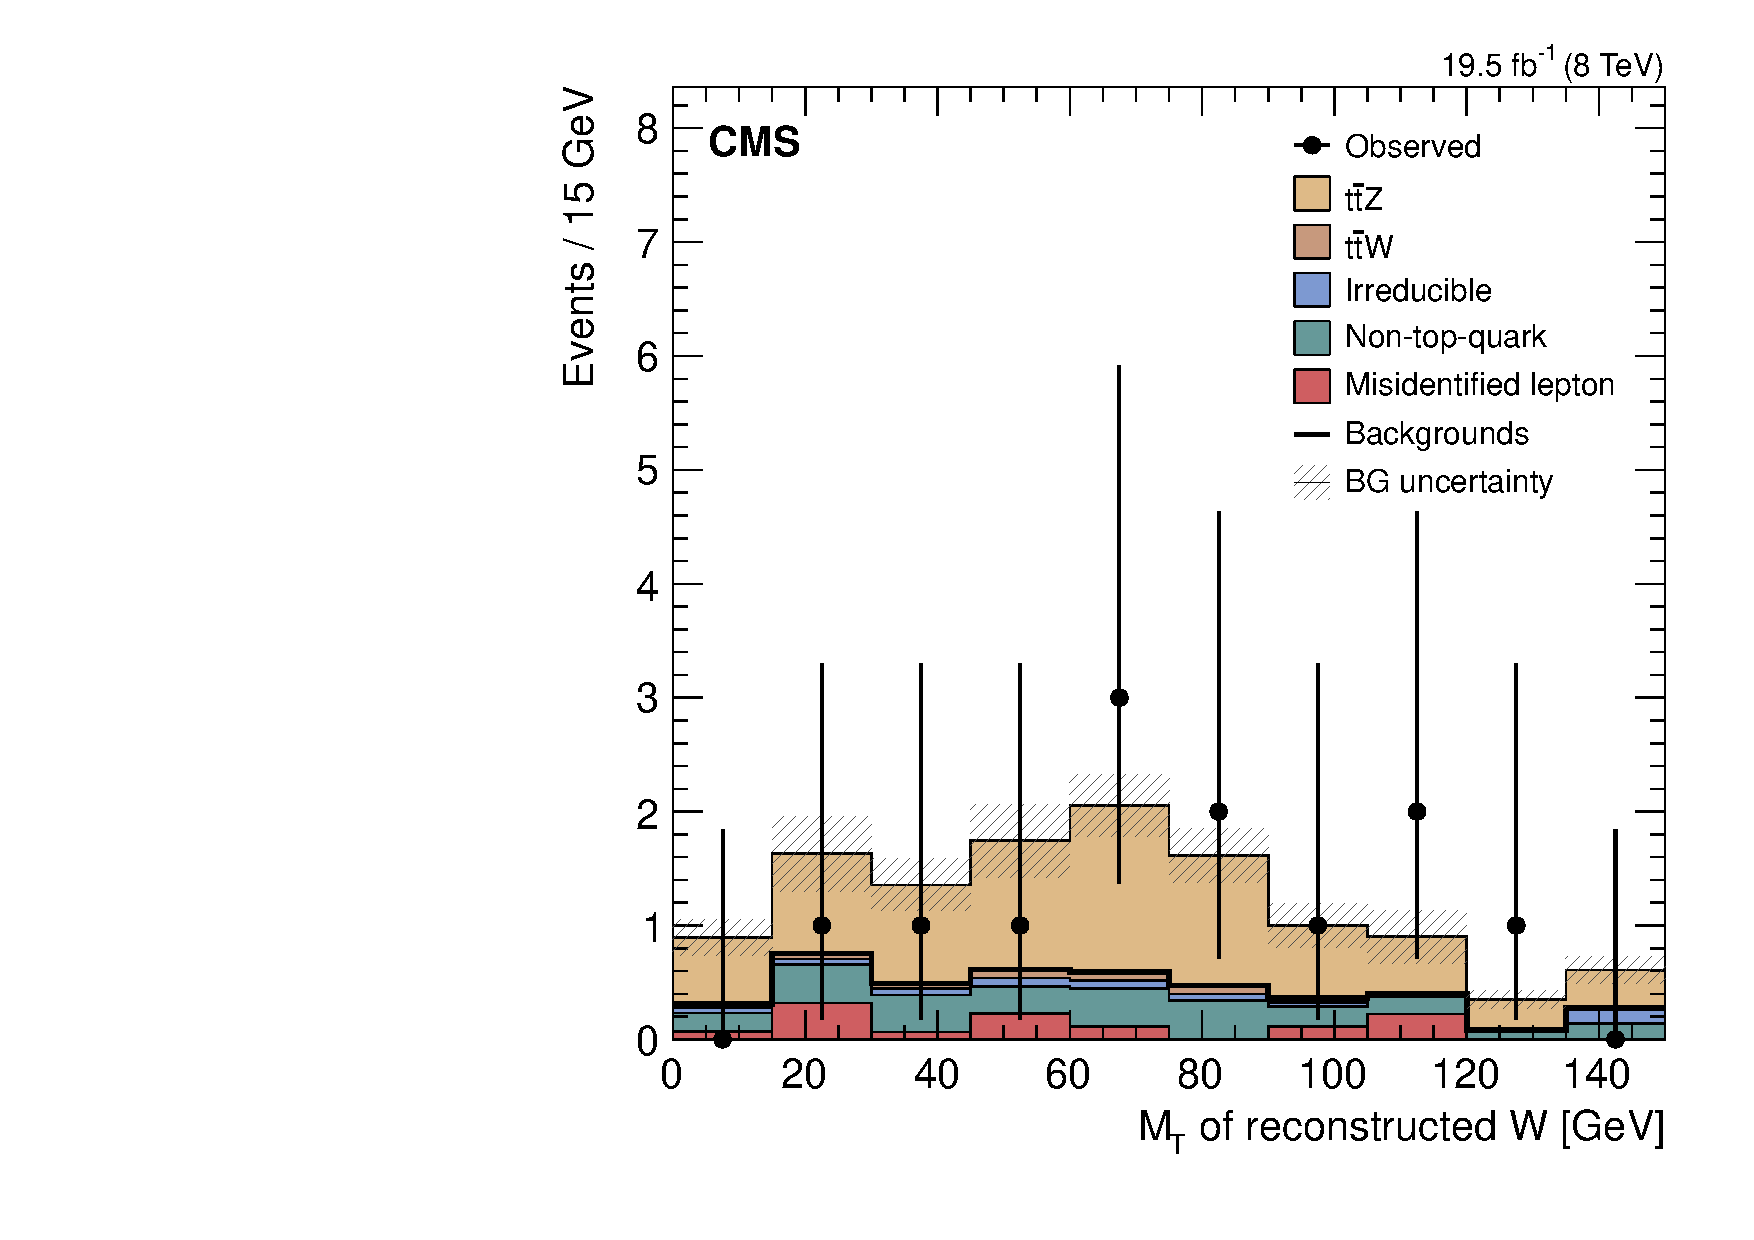
\includegraphics[width=0.48\linewidth]{Figs/Plots_Final_Selections/hWMt_3L2J2b.pdf}
\caption{\label{fig:hmass_3l2j2b}
Reconstructed mass of Z (Left) and \Mt of the W (Right) are shown after all selections have been applied.
}
\end{center}
\end{figure}


Figures ~\ref{fig:hpfMET_3l2j2b} and ~\ref{fig:hHt_3l2j2b} show two more defining characteristics. Both the pfMET and \HT \ are important shapes caused by the neutrino produced in the leptonic W decay and the jets produced in the top and hadronic W decay. Since these variables are not used in the current selections, they are plotted to show extra confirmation of the yields.

\begin{figure}[h]
\begin{center}
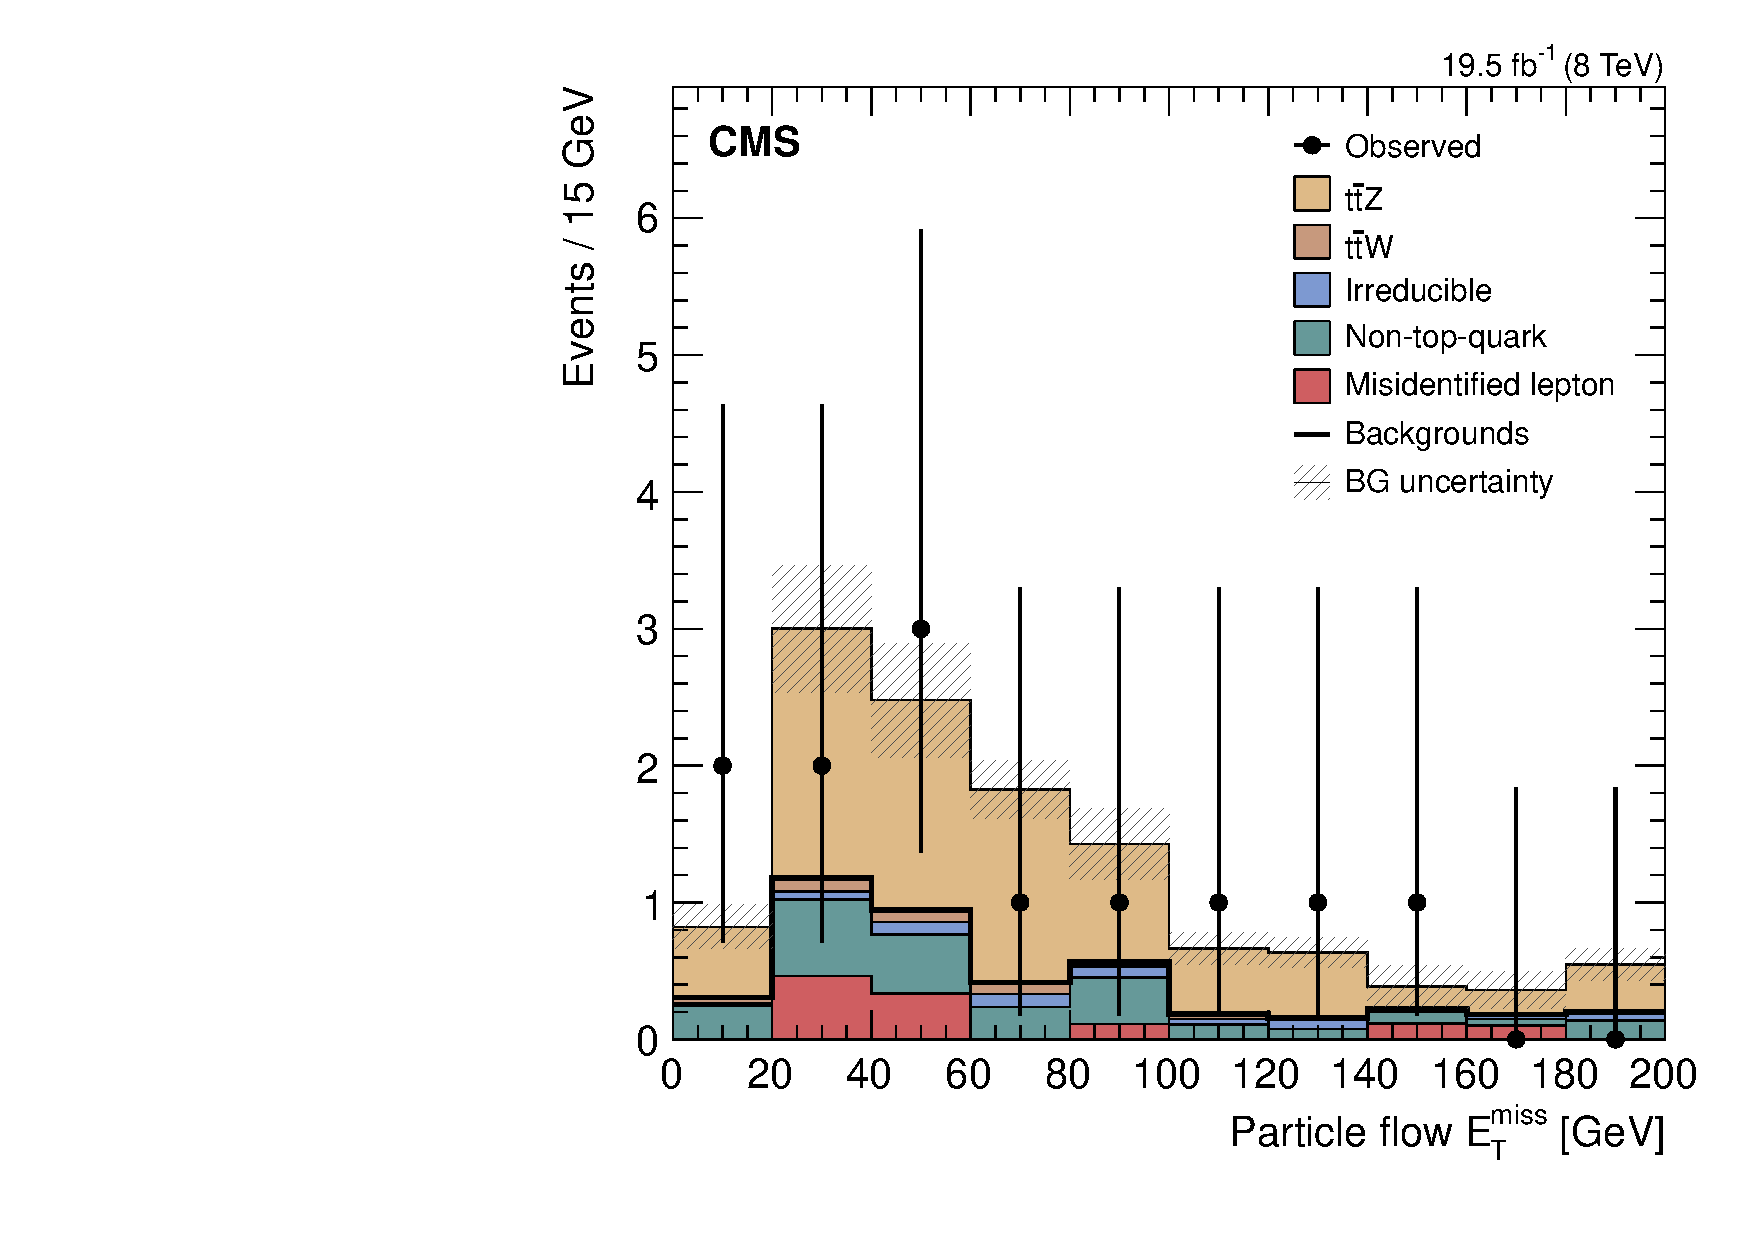
\includegraphics[width=0.48\linewidth]{Figs/Plots_Final_Selections/hpfMET_3L2J2b.pdf}
\caption{\label{fig:hpfMET_3l2j2b}
pfMET of the events after full analysis selections have been applied.
}
\end{center}
\end{figure} 

\begin{figure}[h]
\begin{center}
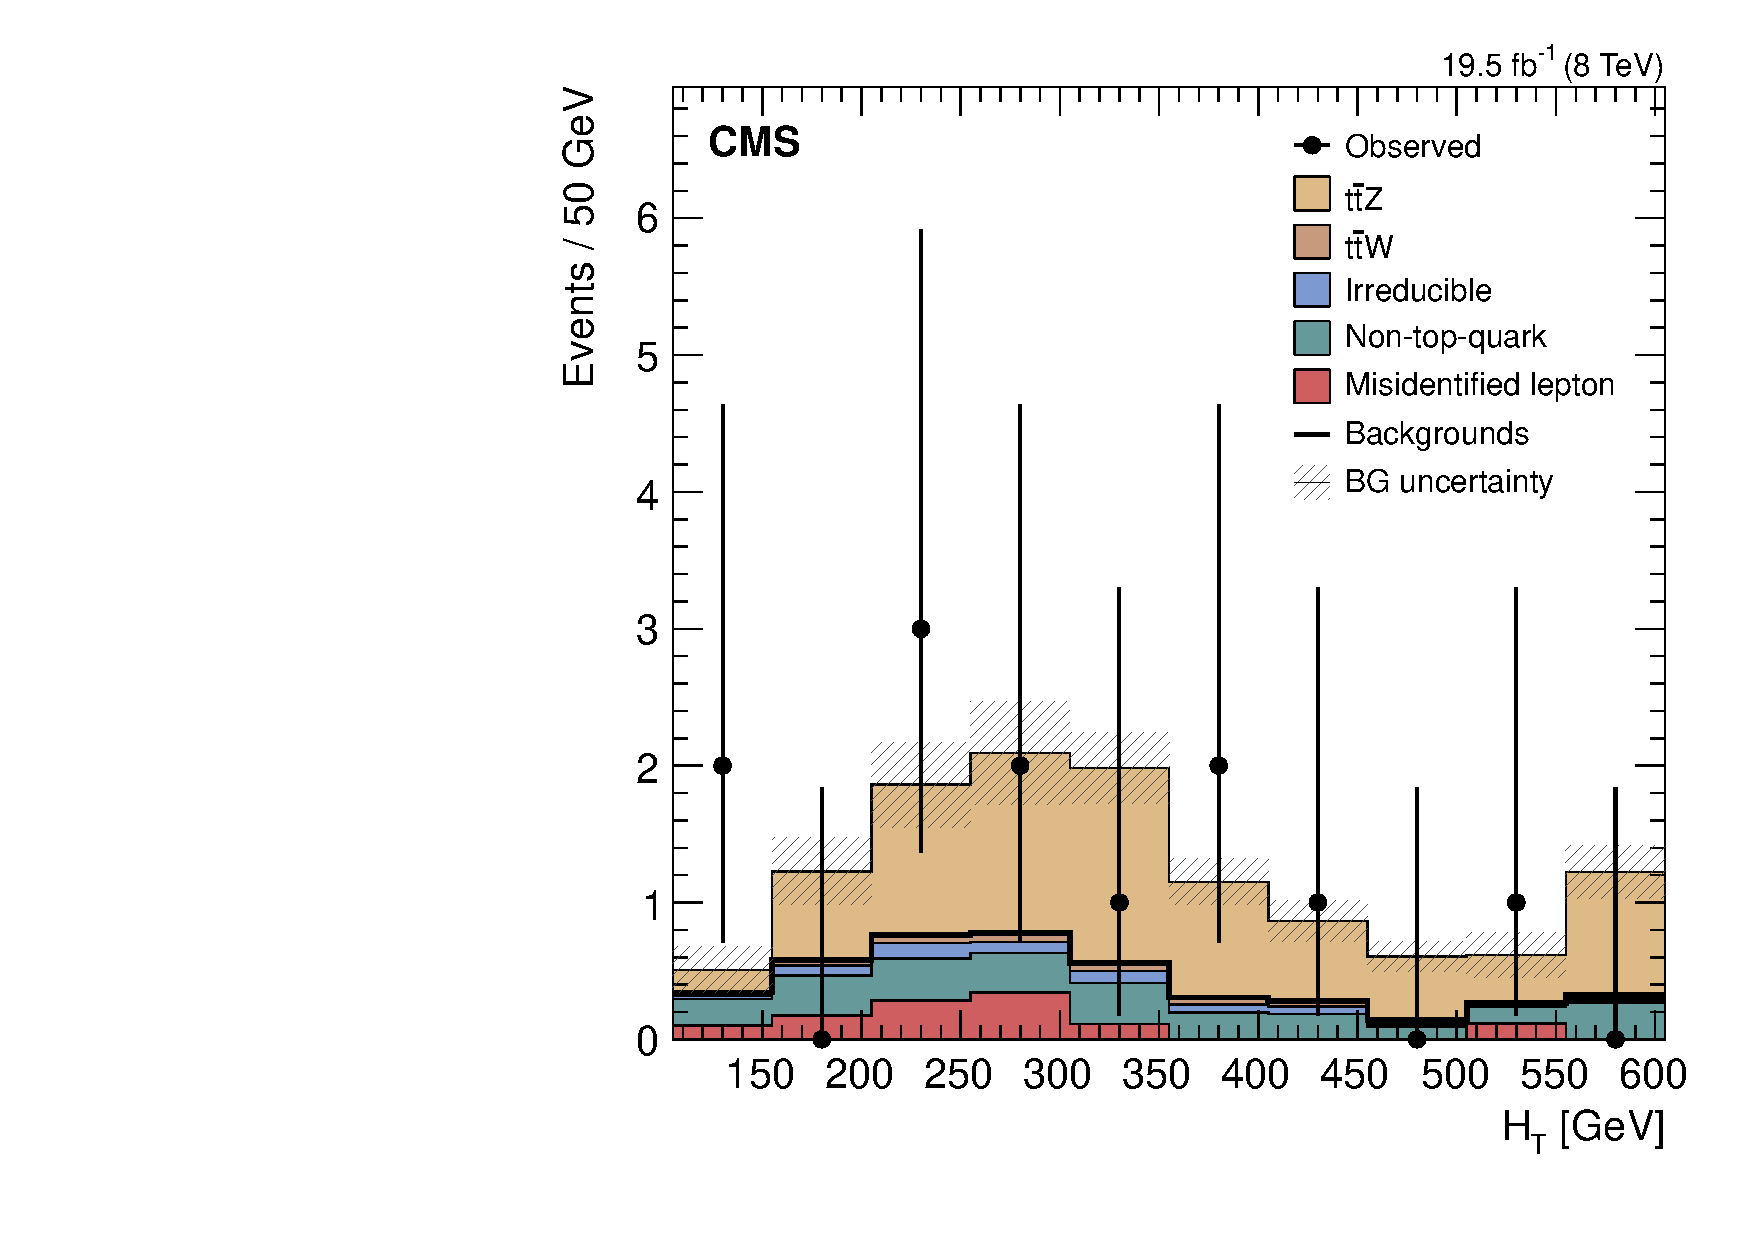
\includegraphics[width=0.48\linewidth]{Figs/Plots_Final_Selections/hHt_3L2J2b.pdf}
\caption{\label{fig:hHt_3l2j2b}
\HT \ of the events after full analysis selections have been applied.
}
\end{center}
\end{figure} 















	
	
	\section{cross section calculation and significance}
	The \ttZ \ signal is estimated in Section ~\ref{sec:signal} to be $7.62 \pm 3.46_{data\ st} \pm 0.73_{bkg\ st} \pm 1.37_{bkg\ sy}$. For the luminosity of the full dataset, we use the quoted luminosity of \intLumiwError ~\cite{lumimeasurement}. Finally, we calculate the Branching Ratio (BR) multiplied by the Acceptance of selections (Acc) multiplied by the Efficiency of selections ($\epsilon$) all at once. To do this, we divide the number of \ttZ \ events in MC (using the sample listed in Table ~\ref{tab:IrreducibleMCSamples}) that pass selections by the total number of \ttZ \ events in MC. This gives a BR $\times$ Acc $\times \epsilon$ of $0.0021 \pm 4.0\% _{st} \pm 10.5\% _{sy}$.\\

The full cross section is given by 
          \begin{align*}
         \sigma &= \frac{Yields - Bkg}{\mathcal{L} \times BR \times Acc \times \epsilon} \\
                      &=  186 \pm 85_{data\ st} \pm 18_{bkg\ st} \pm 33_{bkg\ sy} \pm 7_{BR*Acc*\epsilon\ st} \pm 20_{BR*Acc*\epsilon\ sy} \pm 5_{lumi\ sy}\ fb\\
                      &= 186 \pm 107\ \text{fb}\\
          \end{align*}
          
          
          
 Additionally, the LandS software is used to perform this calculation with a bit more rigor (see ~\cite{higgscomb}). Data cards are prepared from the information contained in this note. Backgrounds are assumed to be log normal with uncorrelated errors. Data driven backgrounds use the statistical and systematic uncertainties that were derived with the methods. Monte Carlo only backgrounds use the uncertainties derived in Section ~\ref{sec:systematic}. With this preparation, the signal strength (Table ~\ref{tab:significance}) and ratio to theory cross section (Table ~\ref{tab:landsout}) are found (where again the NLO theory cross section for \ttZ \ production is 205 fb). The final cross section measurement is $\sigma=194 _{-89} ^{+105}$ \ fb.
 
 
 
\begin{table}[ht!]
\begin{center}
\caption{\small \label{tab:significance} Expected and measured significance of the signal.}
\begin{tabular}{c|c}\hline
	& Significance	 \\ \hline
Expected	& 2.45	 \\
Measured	& 2.33	 \\
\hline
\end{tabular}
\end{center}
\end{table}
 
\begin{table}[ht!]
\begin{center}
\caption{\small \label{tab:landsout} Measured cross section as calculated by LandS.}
\begin{tabular}{c|cc}\hline
	& r        & Cross Section	 \\ \hline
	&  & \\
\ttZ	& $0.94 _{-0.43} ^{+0.51}$ & 	$194 _{-89} ^{+105}$ fb\\
& & \\
\hline
\end{tabular}
\end{center}
\end{table}
 
 
 
 
 Ratio to Theory = $0.94 _{-0.43} ^{+0.51}$\\
	